\documentclass{article}
\usepackage[utf8]{inputenc}
\usepackage[english]{babel}
\usepackage{amsmath}
\usepackage{amssymb}
\usepackage{setspace}
\usepackage{natbib} 
\usepackage{graphicx}
\usepackage{subfig}
\usepackage{comment}
\usepackage[backgroundcolor=pink,linecolor=red]{todonotes}
 \usepackage{fullpage}
\usepackage[hidelinks]{hyperref}
\usepackage{xcolor}


%\singlespacing
\onehalfspacing
%\doublespacing

\newcommand{\plr}[1]{\todo[linecolor=blue,backgroundcolor=blue!25,bordercolor=blue]{#1}}
\newcommand{\jgg}[1]{\todo[linecolor=green,backgroundcolor=green!25,bordercolor=black]{#1}}
\newcommand{\bill}[1]{\todo[linecolor=green,backgroundcolor=yellow!25,bordercolor=black]{#1}}

\begin{document}

\title{The sweet spot for local polygenic adaptation: a case study motivated by stickleback}
\author{Jared Galloway, William A. Cresko, and Peter Ralph}
\maketitle

\textbf{Other title ideas?} (Bad ideas allowed.)

How do stickleback share adaptations between lakes? A simulation study.

A simulation study of gene flow and local polygenic adaptation

\bill{A simulation study of gene flow and local polygenic adaptation in stickleback fish}


\textbf{JARGON WE SHOULD THINK ON ??}

effect loci (locus) | QTL | causal: = ?
 
Original Lakes | initial | $P_{1}$, $P_{3}$, $P_{3}$ = ?

Migration Rate | Historical Introgression = ?

pre-existing freshwater adapted alleles | standing genetic variants = ?


\textbf{Pending things to do?} that maybe we do, maybe not

longer genomes ($10^8$ not $10^5$ but rescaling everything accordingly)

verify that adaptation of introduced pops is due to initial diversity not subsequent migration

\section{Abstract}

Threespine stickleback fish provide one of the most striking examples of local adaptation. This hemisphere-wide metapopulation includes both marine populations and a large number of smaller freshwater populations
that have apparently repeatedly adapted to freshwater conditions
often using the same genetic basis.
In this paper, we use simulations motivated by stickleback populations
to examine what amounts of gene flow favor stable metapopulation polymorphism
with allele sharing,
and to further dissect the underlying dynamics.
We find that rapid, repeated adaptation 
using alleles maintained at low frequency by migration-selection balance
(the ``transporter hypothesis'')
occurs over a realistic range of intermediate rates of gene flow,
between slow, independent adaptation with low gene flow
and large migration load at high gene flow.
This is mediated mainly by the total downstream influx of alleles \emph{(maybe??)}.
We do not see evidence for strong effects encouraging genomic clustering of causal alleles
or towards particular dominance coefficients.
$F_{ST}$ scans for adaptive alleles are more likely to succeed with higher rates of gene flow,
The results support existing theory of local adaptation,
and provide a more concrete look at a particular, empirically motivated example.


\section{Introduction}

% Jared's general notes for formatting
%
% - ``citep'' for ``cite in parentheses''. (and, citations come before the punctuation)
% - in latex, use ` `words' ' to get the open- and closed-double quotes (not the double-quote character)
% - "citet" for "cite, as part of the text"

\emph{intro outline:}
Start off with stickleback: repeated, rapid, parallel adaptation with obvious phenotypes.
But, most species don't seem to have such obviously structured polymorphism: 
what's special about stickleback?
The transporter hypothesis is a mechanism; what's required to make it work?
Other species adapt rapidly in similar ways:
e.g., Darwin's finches and island mice;
do these differ through not having such a big, connected reservoir of genetic variation?
or by not having such a large total population size of the ``other'' habitat?
Or, is this situation more common than we know, with less obvious phenotypes?
Also, can we actually tell what's happening from genetic data?

Recently, multiple instances of similar (parallel) underlying genetic basis of rapid local adaptation has brought about 
questions surrounding the origins and maintenance of genetic polymorphism.
A empirical model is the Alaskan populations of freshwater and marine Ninespine Stickleback fish.
In 1964, The Great Alaskan Earthquake caused an uplift of Middleton island and in turn,
introduced a group of freshwater ponds around the perimeter of the island. 
Quickly inhabited by the surrounding marine population of Stickleback,
\citet{lescak2015evolution} observed significant phenotypic changes in less than 50 years that appear to be 
parallel to freshwater stickleback that have been separated for over $13,000$ years.
In freshwater stickleback, the number of lateral plates are reduced
and the opercle shapes shows the same expansion of the dorsal region and reduction of the ventral region.
% \jgg{Bill - more specifics about Bill, Suzie, Kristin  \& or Thom's papers .. ? }
These results leave us with questions surrounding the nature of rapid adaptation.
Does convergent evolution breed it's own solution (haplotype) for every new selective pressure, 
or can these solutions can be efficiently shared across multiple sub - populations facing similar selective pressures. 

The leading hypothesis for stickleback is that rather than acting on new mutations, 
adaptation to freshwater environments is sped up through selection on standing genetic variation (SGV) found in marine populations. 
\jgg{Bill: maybe you could make this section a little more specific}
One clear example of this is the gene \textit{eda} 
which has been shown to regulate the number of lateral plates. 
While this gene arose millions of years ago, it is found in freshwater ponds which have formed much more recently.
Novel evidence from natural populations has provided evidence that most regions of the genome that distinguish marine-freshwater genetic differences share this pattern \citep{nelson2017ancient}.
\citet{schluter2009genetics} 
suggested the ``transporter''-hypothesis.  
This outlined the flow of freshwater alleles into marine populations through offspring of hybridization events.
It suggests freshwater haplotypes are distributed though marine individuals and are continually selected upon in introduced freshwater populations.
The continued selection on freshwater favored alleles and introgression between the two sub-species,
allows the marine to maintain the freshwater haplotype dispersed in low frequency among its' individuals. 
Once a new freshwater environment is introduced and inhabited by marine individuals who carry freshwater adapted alleles, selection reconstructs the freshwater haplotype \citep{schluter2009genetics}.
An alternative to this hypothesis is that individuals from other freshwater environments migrate directly to the new environments, 
and their haplotype is passed down directly. 
This hypothesis has been shown to be unlikely due to finding a high frequency of freshwater alleles in the ocean,
and almost no freshwater individuals.

\plr{Bring up the possibility of more than one freshwater haplotype here.}
\jgg{Re: should I? Doesn't Thom's work and parallel above suggest they have the same alleles?}

If selection on standing genetic variants is key in rapid adaptation, 
many questions are exposed concerning the surrounding population genetics parameters and underlying genomic architecture.
%How rapidly can selection act on standing genetic variants at a given value of migration, $M$?
What scale of historical introgression between populations with selective pressures $X$ and $Y$, allows for rapid and parallel local adaptation
of a population derived from $X$ to an introduced environment with selective pressure $Y$?
What is the origin of pre-existing adaptive variants?
How are the variants structured, historically and across the genome underlying the trait?
%How does population genetics data influenced by historical introgression and selection on standing genetic variants?
%How many alleles underly a certain trait and how many are swept away by drift? 
Furthermore, how can we infer causal loci for regions of the genome that must be driving the rapid adaptation, from real data.
Many biologists today make use of genome wide association studies (GWAS) and 
$F_{st}$ across the genome to estimate regions responsible for certain traits. 
Unfortunately, the data can be heavily influenced by the level of introgression and population structure of the samples. 
This being the case, what are the biases we can expect to see in real data for certain levels of introgression. 

There are many different parameters that carry a large impact on the questions above.
\citet{ralph2015convergent} 
explored the dichotomy of selection on new alleles and those brought in by migrants from a similar selective pressure.
Answering the fundamental questions surrounding spatial resolution of convergent evolution. 
%This lead to an understanding of the process by which alleles move from an existing 'patch' to an introduced 'patch' with the 
%same selective pressure. 
\jgg{It seems like this could be a good parallel to what we're doing here, or maybe for discussion?}

In this paper, we explore time to local adaptation as a function of migration rate through an environment (marine) with opposing selective pressure. 
Next, we compare to real data and explore how $F_{st}$ data can be impacted by introgression.
%Explain what we do and what we find that is important

%We use forward moving simulations to model marine and freshwater populations of stickleback.
%We then observe the effect (focusing on migration and recombination, for now) 
%of different parameters on local adaptation of introduced freshwater environments. 


%%%%%%%%%%%%%%%%
\section{Methods}

We explored these questions
using forwards-time simulations with explicit genomic representation of a quantitative trait
in SLiM \citep{haller2017slim}.
The details (described below) are motivated by previous population genomic studies of threespine stickleback,
but remain simplistic in some aspects due to computational constraints.
Possibly the most important caveat is that simulated population sizes are much smaller
than the census size of the threespine stickleback population;
we will consider the likely effects of this in the Discussion.
\plr{TODO}


\paragraph{Habitat and geography}
Our model has two habitat types, which are considered separate populations
with a fixed total size of 2,000 diploid individuals each. The marine population is treated as a single large deme, but the freshwater population is subdivided into local subpopulations or demes.
The scheme, depicted in Figure \ref{fig:Geo},
roughly models a set of freshwater habitats
along a stretch of coastline.
The ``marine'' habitat  is a continuous, one-dimensional range of 10 units of length,
and the ``freshwater'' habitat is divided into ten subpopulations
(which we call ``lakes''), each connected to the marine habitat
at positions $i - 1/2$ for $1 \le i \le 10$.

Fitness in each habitat is determined by a single continuous trait with an inherent tradeoff such that alternative values of the trait have high or low fitness in tht two different habitats. This situation roughly models the cumulative effect of the various phenotypes
such as armor morphology, body size, craniofacial variation and opercle shape (among others)
on which divergent selection acts in the two environments.
The optimal trait value in the marine habitat is $+10$,
and in the freshwater habitat is $-10$. Fitness of a fish with trait value $x$ in a habitat with optimal value $x_\text{opt}$ is
Gaussian with standard deviation, i.e.,
\begin{align*}
    f(x; x_0)
    &=
    \exp\left\{
        \frac{1}{2}
            \left(
            \frac{x-x_\text{opt}}{15}
            \right)^2
        \right\} .
\end{align*}

\begin{figure}
	\begin{center}
  		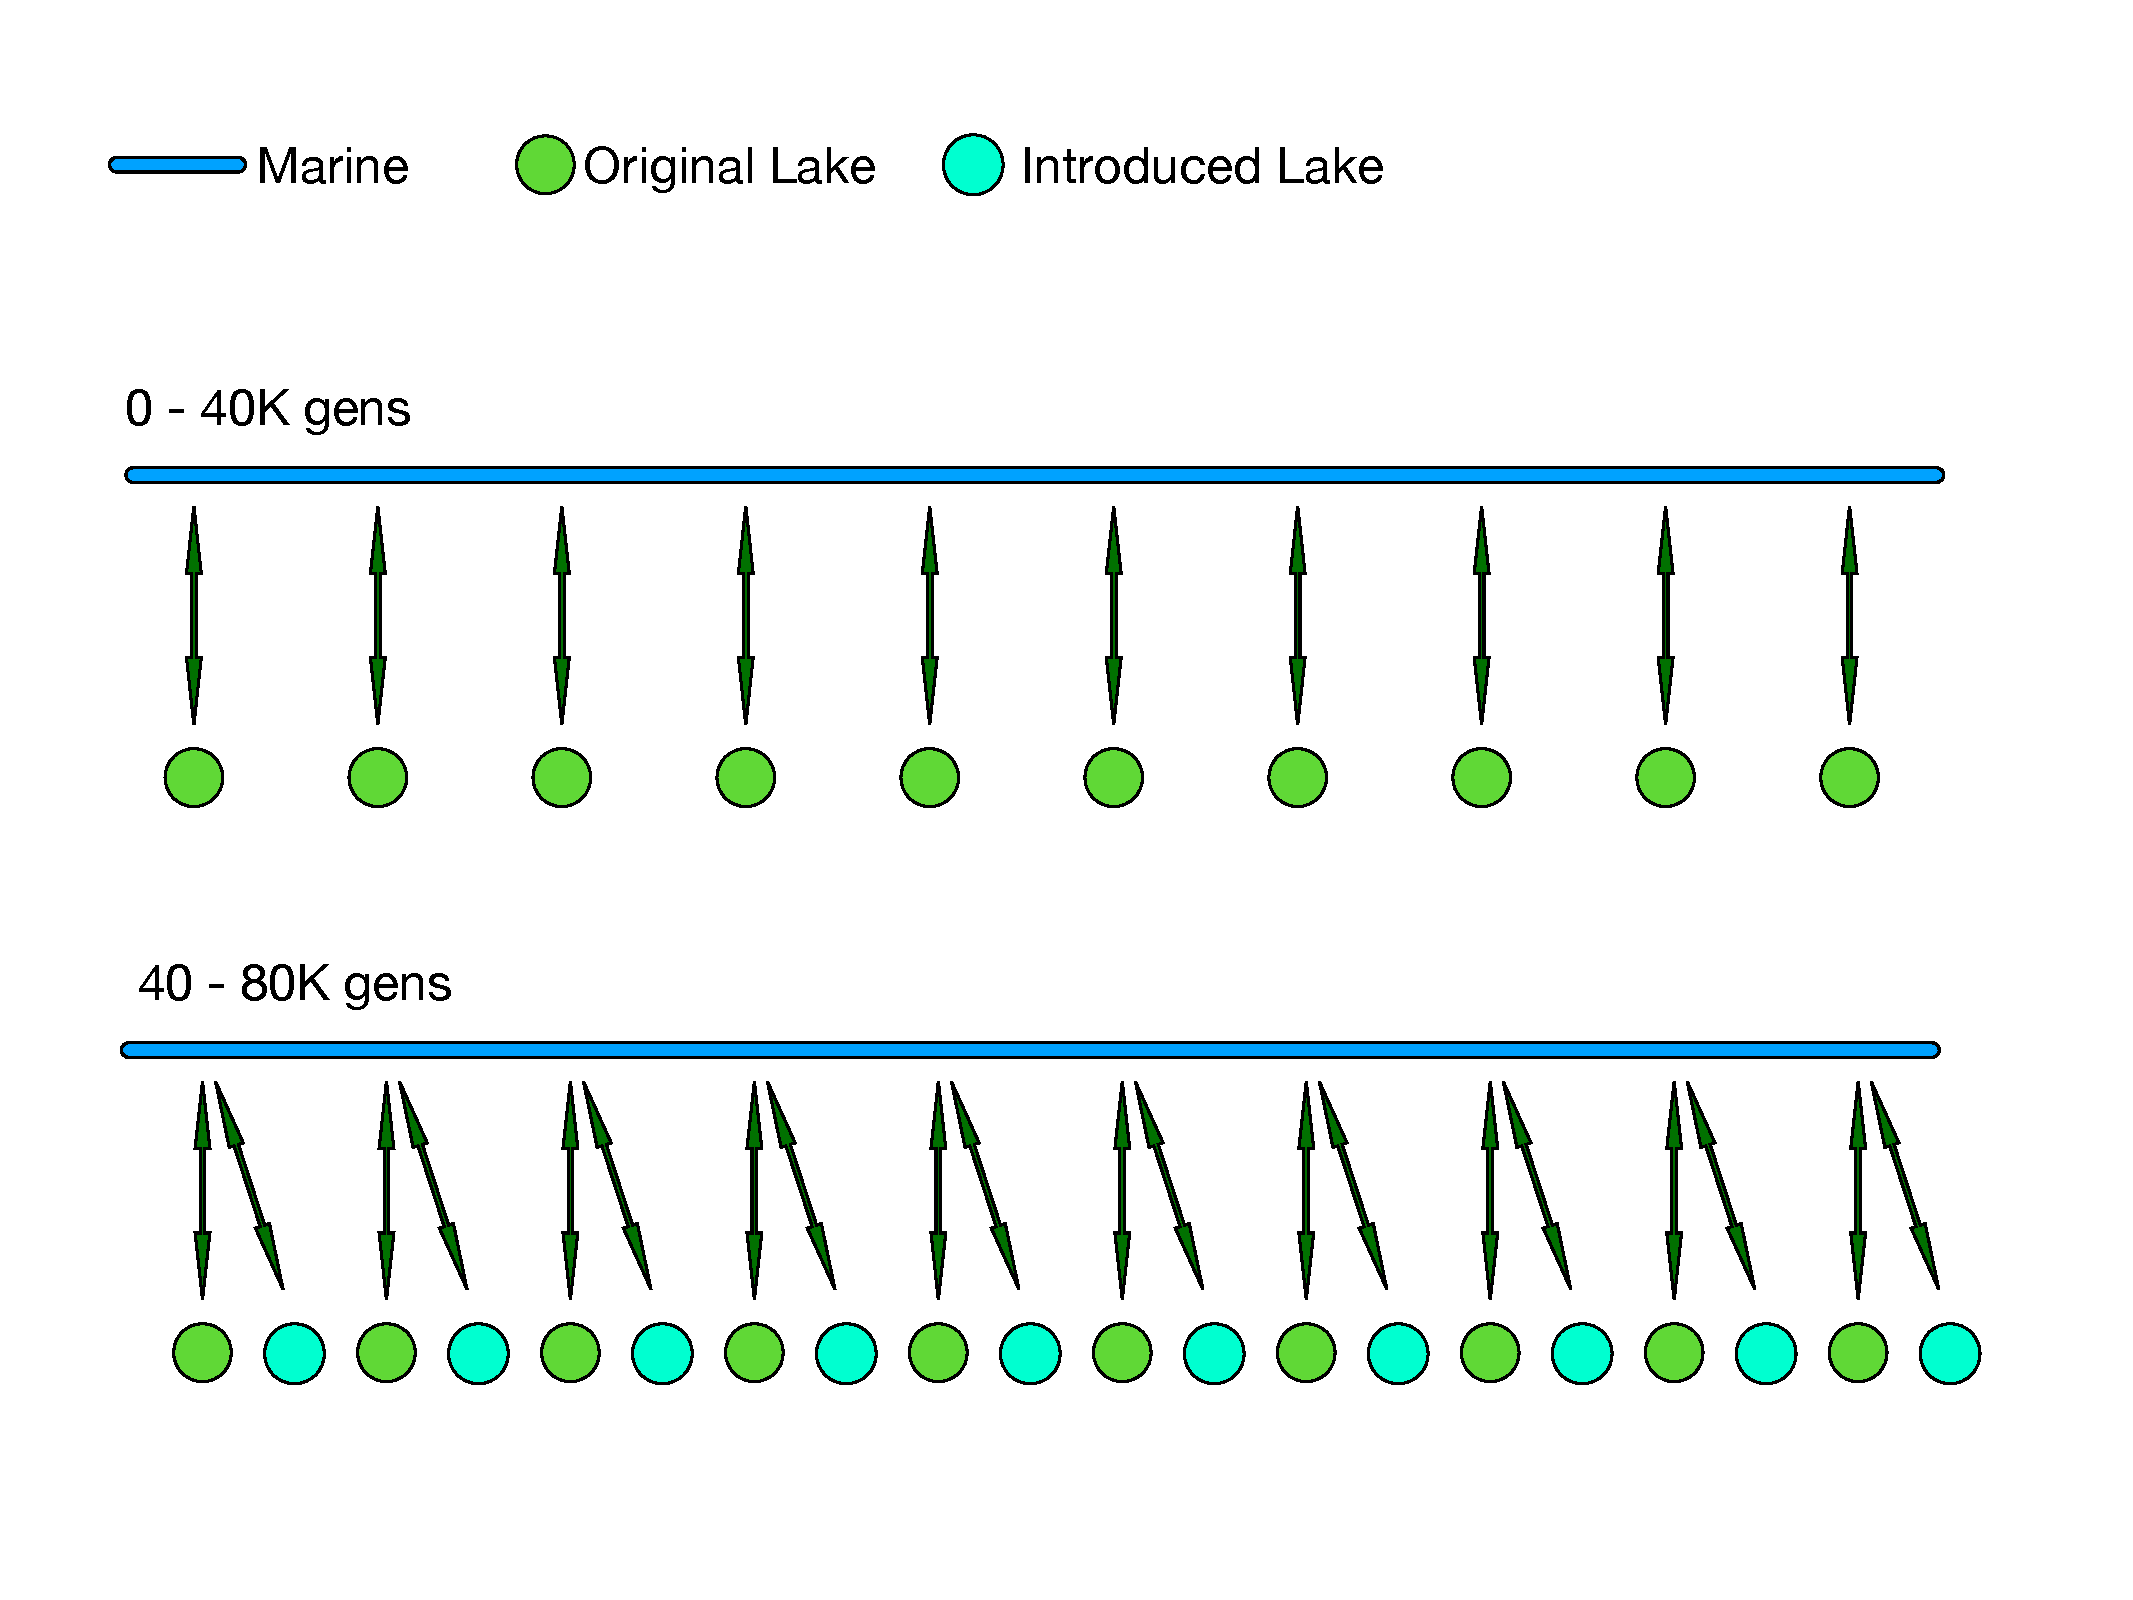
\includegraphics[width=0.6\linewidth]{GeographyDiagram}
  		\caption{A representation of the geographic and evolutionary history of all populations throughout the simulation. 
		The marine is a one-dimensional, continuous population with spatial positions ranging from [0.0 - 10.0]. 
		Each freshwater lake$_{i}$ for both the introduced and freshwater populations
		is a discrete population connected by migration only through the marine, at position $i - 0.5$. 
		The introduced lakes have the same spatial location (but separate?) and selective pressure as the original lakes, but arise at 40K generations.
		The marine has $2000$ diploid individuals while each of the lakes fluctuate around $200$. 
		the introduced population is initialized as a copy of all marine individuals to model marine 
		individuals inhabiting a newly created freshwater environment such as the ponds around Middleton Island.
		We then observe the selection process of marine individuals and following generations 
		with the new selective pressure across a range of parameter values. 
		%Migration between the marine and original lakes is 
		%set to $0$ the generation before introduction to avoid direct migrants from original $->$ introduced lakes.
		}
  		\label{fig:Geo}
	\end{center}
\end{figure}


\paragraph{Potential genomic architecture}\bill{Initial genomic architecture? The header is a little confusing to me}
Each individual carries two copies of a linear chromosome of $10^5$ loci
(which could be thought of roughly as a kilobase each).
New mutations occur with probability $10^{-7}$ per locus per generation.
Ten ``effect regions'' of 100 loci each
are spread evenly along the chromosome (separated by 4950 loci)
in which mutations affect the trait;
mutations in other parts of the genome are neutral.
Each mutation in these regions is either additive, completely recessive,
or completely dominant (with equal probability),
and with an effect sizes chosen randomly from an Exponential distribution with mean $1/2$,
either positive or negative with equal probability.
Individual trait value are determined additively from the diploid genotypes.
Concretely, an individual that is heterozygous and homozygous for mutations
at loci $H$ and $D$ respectively
has trait value
$x = \sum_{\ell \in H} h_\ell s_\ell + \sum_{\ell \in D} s_\ell$,
where $s_\ell$ is the effect size of the mutation at locus $\ell$.
Subsequent mutations at the same locus replace the previous allele.

\paragraph{Life cycle}
Each generation, the two parents of each new offspring are chosen 
proportional to their fitness (all individuals are hermaphroditic),
and the contributing genomes are produced by Poisson recombination
with an average of one crossover per chromosome per generation
($10^{-7}$ per locus per generation).
The model is Wright-Fisher, so that each generation, in each habitat,
2000 new individuals are produced,
and so to keep population sizes roughly constant within each lake,
at the start of each generation we rescale fitness values in the freshwater habitat
so that the sum of the fitness values within each lake are equal.

Migration occurs both locally along the coastline in the marine habitat
and between the marine habitat and the lakes,
and can be thought of as occurring at the juvenile stage.
The between-habitat migration rate is denoted $m$,
and will be called simply the ``migration rate''.
Each new individual in the marine habitat has freshwater parents with probability $m$;
to obtain the pair, a first parent is chosen proportional to fitness,
and a mate is chosen from the same lake as the first, also proportional to fitness.
The resulting offspring is given a spatial location in the marine habitat
at the location of the parent's lake.
Parents for a new marine individual who is not a migrant are chosen similarly (with probability $1-m$):
first, a single parent is chosen proportionally to fitness in the marine habitat,
and then a mate is chosen, 
also proportionally to fitness but reweighted by a Gaussian function 
of the distance separating the two, with stanadard deviation $1/2$. 
Concretely, if the first parent is marine individual $i$,
then marine individual $j$ is chosen as the mate
with probability proportional to $f(x_i) \exp(-2d_{ij}^2)$,
where $d_{ij}$ is the distance between the two locations.
Finally, each new marine offspring is given a position 
displaced from the first parent's position by a random Gaussian distance
with mean 0 and standard deviation 0.02, and reflected to stay within the population.
New offspring in the freshwater habitat are chosen in the same way,
except the probability that the parents are marine individuals is $m$;
any new freshwater offpsring produced by marine individuals
are assigned to the lake nearest to the position of the first marine parent.

\paragraph{New lakes}
To study adaptation in newly appearing freshwater habitats,
we introduce a new set of lakes midway through the simulation.
The initial set of individuals have parents chosen as above from the marine habitat,
and act like an independent copy of the original set of lakes -- in particular,
the two sets of lakes each have 2,000 individuals at all times.
Since this doubles the number of lake-to-marine immigrants,
after this happens the probability that a new marine individual has freshwater parents
is $2m$ instead of $m$.


\paragraph{Descriptive statistics}\bill{Population genetic analyses? Instead of the more general 'Descriptive statistics'?}
To assess whether new lakes adapt using existing genetic diversity,
we define a \emph{pre-existing freshwater adapted allele}
to be an effect mutation that has frequency higher than $0.5$ in at least one of the original lakes,
while remaining lower than $0.5$ in the marine. 
This categorization is made for each generation using the allele frequencies from that generation,
and so changes with time.
Alleles common in the newly introduced lakes do not count
if they are not also common in the original lakes.
They are defined this way because the transportation hypothesis 
does not specify where or when an advantageous mutation arises,
but simply suggests that any sufficiently common freshwater adapted allele 
could participate in adaptaiton in new habitat \citep{schluter2009genetics}.

\emph{Time to adaptation} of the introduced population, denoted $T_\text{adapt}$, 
is defined to be the generation at which 
the difference between the average trait value in the original and the introduced freshwater populations 
is less than 0.5. 

We describe overall genetic differentiation between the habitats using $F_{ST}$,
calculated on a per-locus basis.
Concretely, if $p_f$ and $p_m$ are the frequencies of a given mutant allele
in the freshwater and marine habitats, respectively,
and $\bar p = (p_f + p_m)/2$,
then we compute $F_{ST}$ for that mutation as $1 - p_f p_m / (\bar p (1-\bar p))$.


%%%%%%%%%%%%%%%%%
\section{Results}

% Overview
We varied the migration rate, $m$,
from $5 \times 10^{-5}$ to $5 \times 10^{-2}$ per individual,
i.e., between 0.01 and 10 migrants per year to and from each of the ten lakes.
This had a strong effect on many aspects of adaptation,
including how fast adaptation occurred in each lake,
how much alleles were shared between lakes,
and the population genetic signals left behind.
At the lowest migration rate, lakes adpated nearly independently,
while at the highest migration rate, the habitats are beginning to act like a single metapopulation
with substantial migration load.
We will now dissect what happens between these extremes.

\emph{merge with the above}
Interestingly, the ability for separate populations to locally adapt to their own selective pressure was relatively unaffected 
until the highest rate of migration between the marine and freshwater environments.
All rates of historical introgression aside from the lowest, helped both the initial and introduced freshwater populations 
share pre-existing freshwater adapted alleles.
The sharing of alleles resulted in rapid adaptation ($\approx 100$ generations) of the introduced population (split from the marine population) to adapt to the freshwater environment.
We also found that larger amounts of migration allow for more statistical power and less false positives in the resulting population genetics data ($F_{st}$ per SNP across the genome).



%%%%%%%%%%%%%%%%%%%%%%%%%%%%%%%%%%%%%%
\subsection*{Local Adaptation: differentiation with gene flow}

% The progression of adaptation. How you can see introduction new alleles

Local adaptation occurred in all simulations:
as shown in Figure \ref{fig:phenotype_ts2},
freshwater and marine populations diverged
until the trait means were close to the optimal values in each habitat. 
(Remaining simulations are shown in Figures \ref{fig:phenotype_ts1} and \ref{fig:phenotype_ts4}.)
Greater migration decreased adaptedness only weakly
except for at the highest migration rate (10 migrants per generation per lake),
where the mean trait value equilibrated at roughly half its optimal value 
(Figures \ref{fig:MeanPhenotype} and \ref{fig:phenotype_ts4}).
The establishment of new alleles in the lakes is visible in Figure \ref{fig:phenotype_ts2}
as jumps in the mean trait value;
in the two simulations these occur on a time scale of 100 (lower migration) to 1000 (higher migration)
generations,
and move the trait by an amount of order 1.
Trait variation within each population was small compared to the difference between populations,
with interquartile ranges of around XXX.\plr{TODO}
Across all parameter values, differences at around 16 commonly polymorphic sites 
(eight the shift the trait in each direction)
were responsible for most of the adaptive differences between freshwater and marine habitats.
\plr{ALSO TODO: CHECK THIS}

\begin{figure}
	\begin{center}
        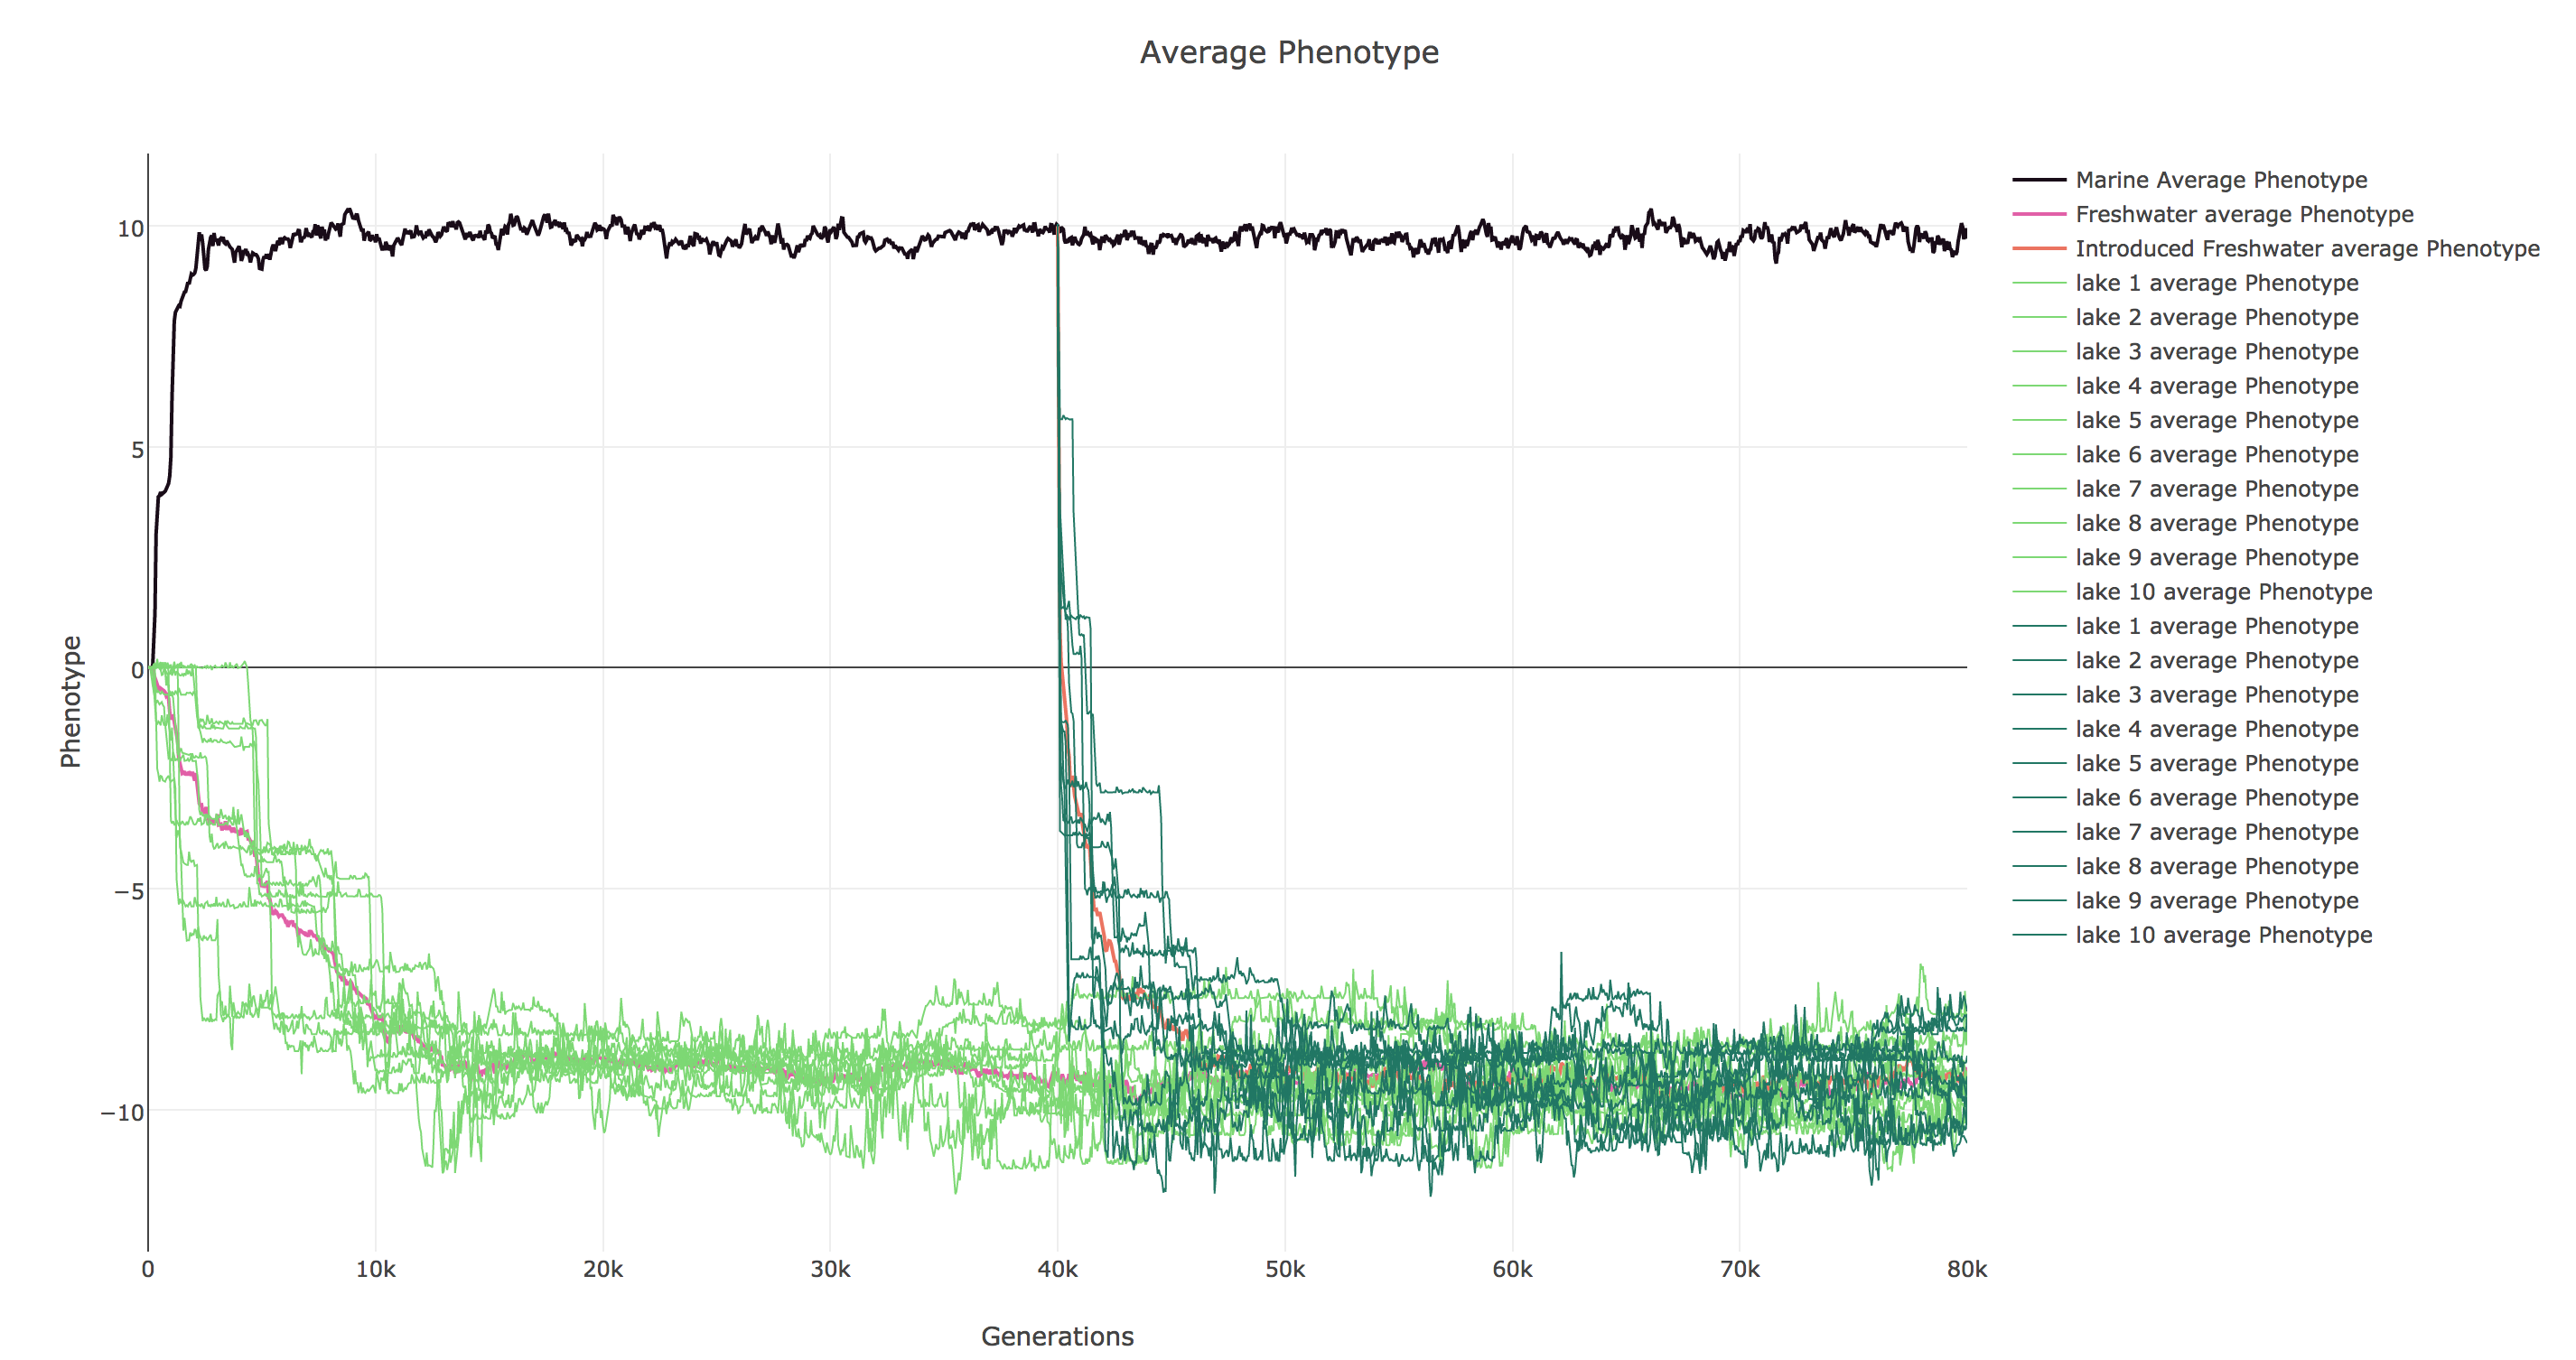
\includegraphics[width=0.7\linewidth]{plotlyPlots/PhenotypeThroughout5e-4}
        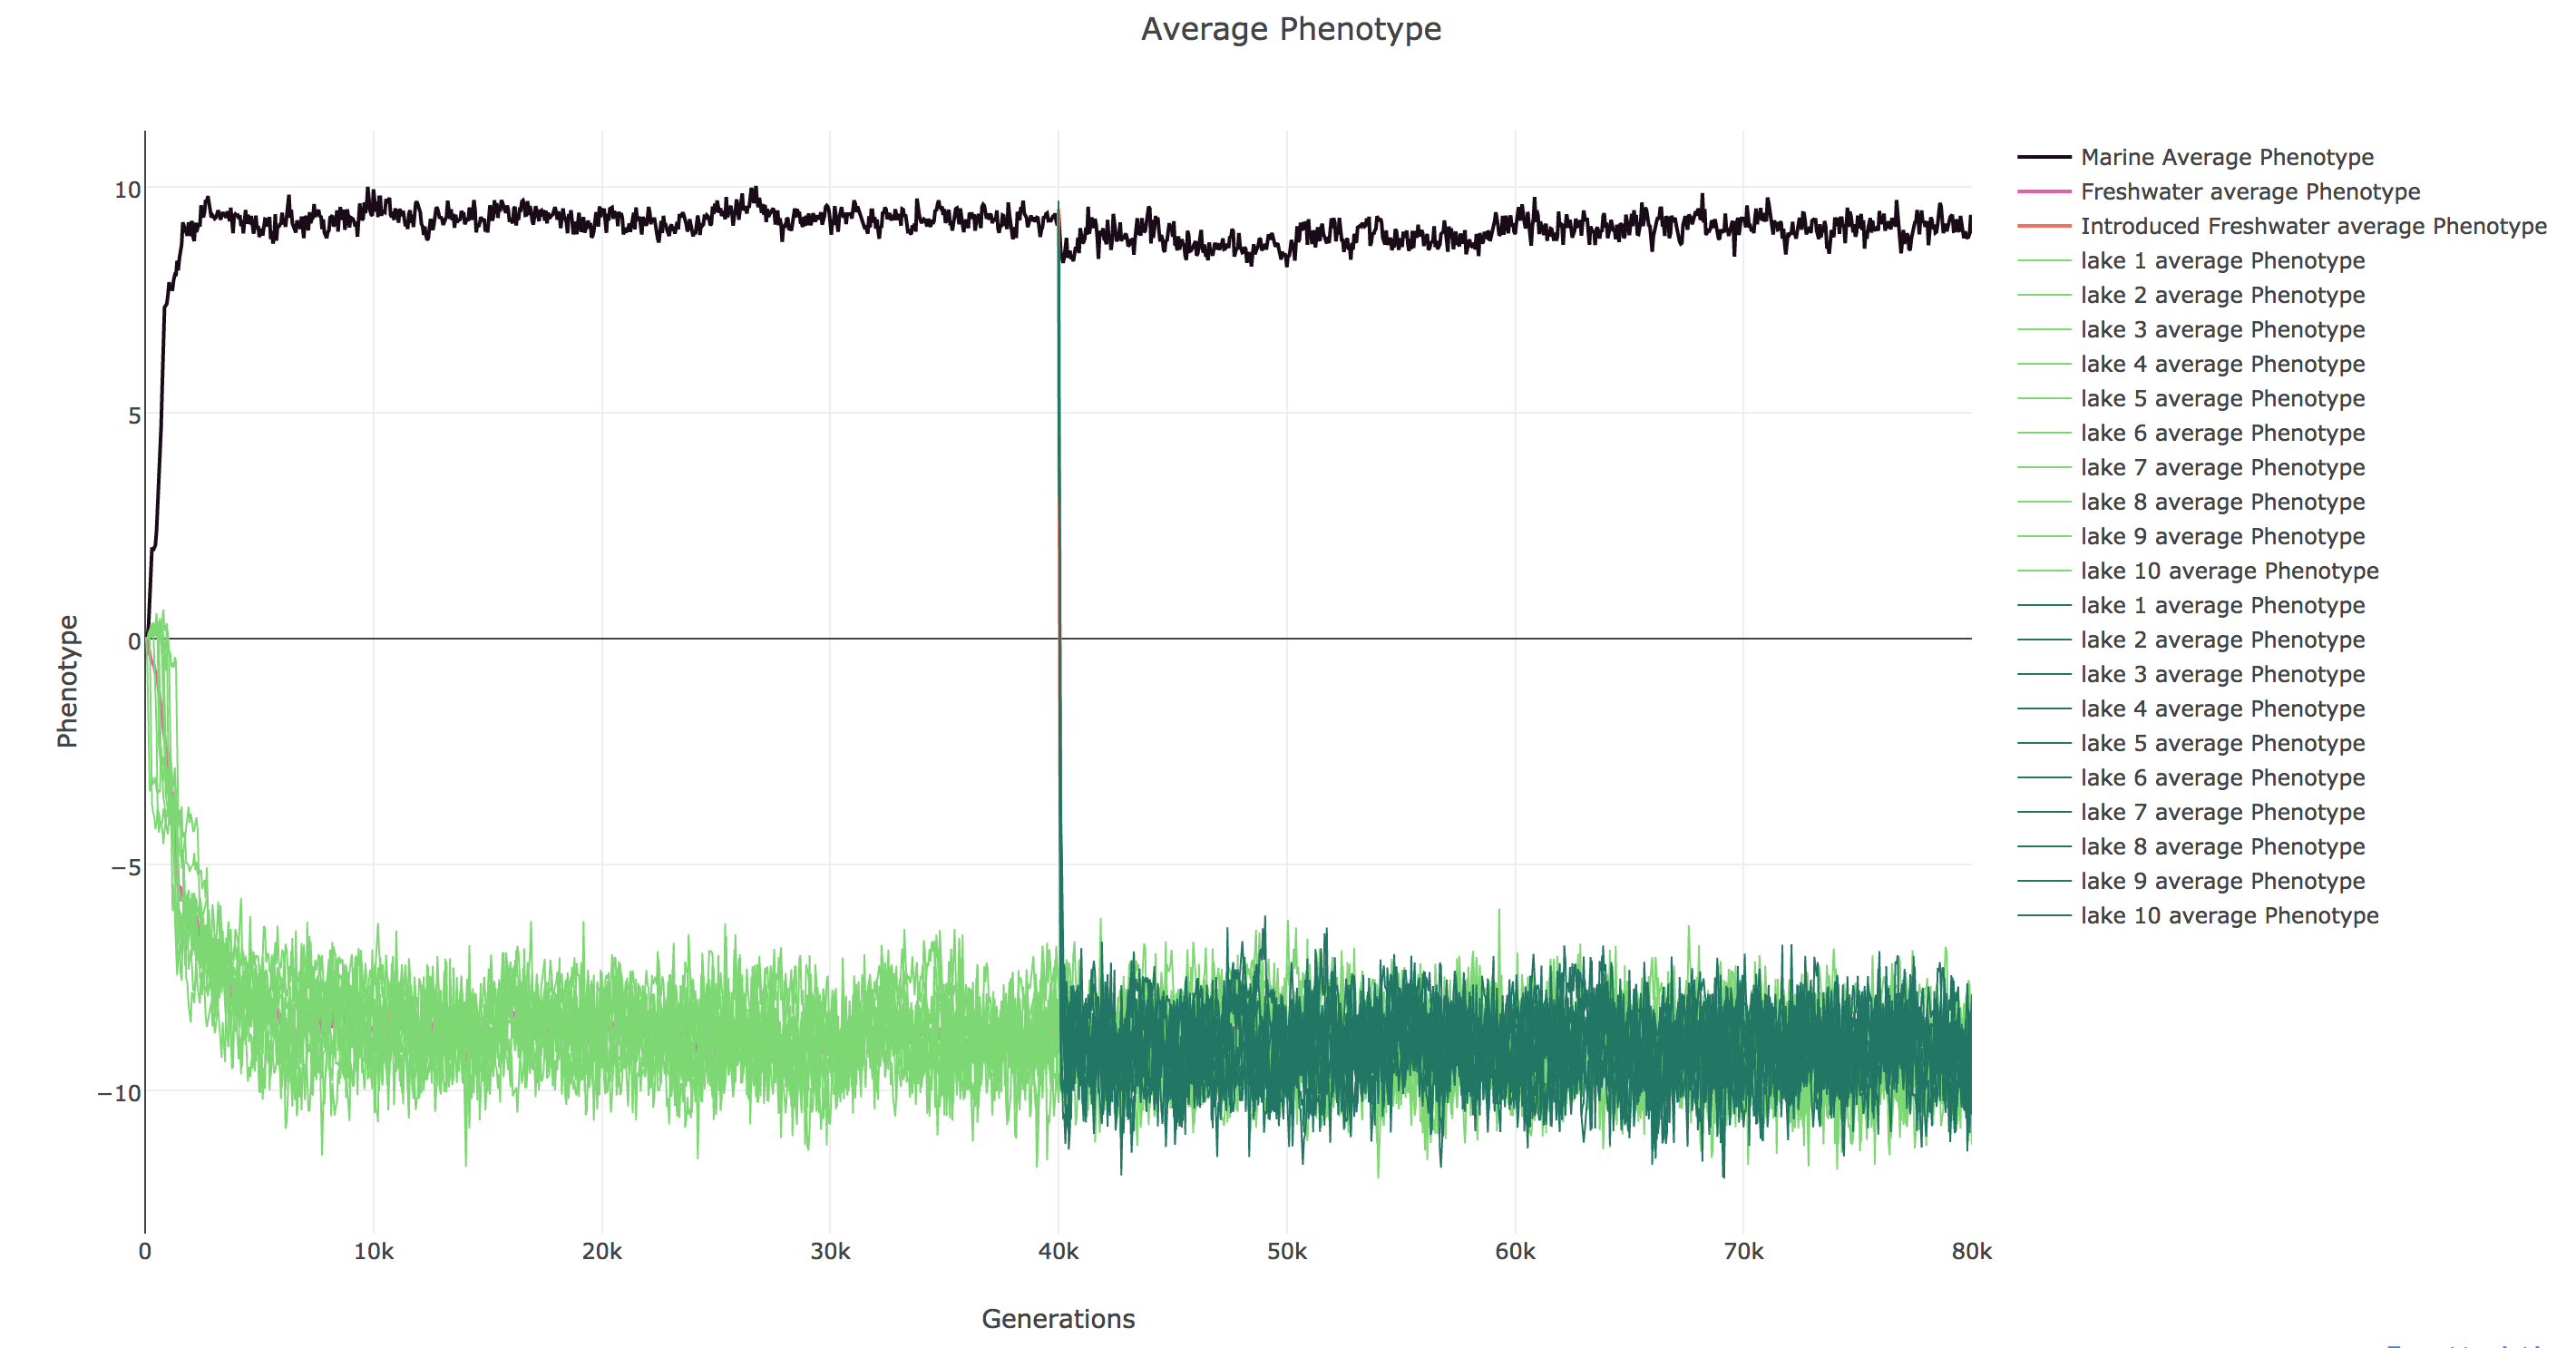
\includegraphics[width=0.7\linewidth]{plotlyPlots/PhenotypeThroughout5e-3}
  		\caption{ 
        Mean individual trait values in the marine habitat (black line),
        the original lakes (light green lines; average in pink),
        and the introduced lakes (dark green lines; average in orange)
        across the course of two simulations, with migration rates of
        \textbf{(top)} $m=5 \times 10^{-4}$ and
        \textbf{(bottom)} $m=5 \times 10^{-3}$ per generation individual
        (i.e., 0.1 and 1.0 migrants per generation per lake, respectively).
        Optimal trait values in the two habitats are at $\pm 10$.
		}
  		\label{fig:phenotype_ts2}
	\end{center}
\end{figure}

\jgg{also, interesting point to make on second plot, you can see the initial lakes taking the same size step, showing sharing of alleles.
could zoom in on the relevent portions of the figure for this. (begging and introduction)
 a 2 by 2 with the important sections (0 - 20K) or (40-50K) for both above figures?}

\begin{figure}[h!tb]
	\begin{center}
  		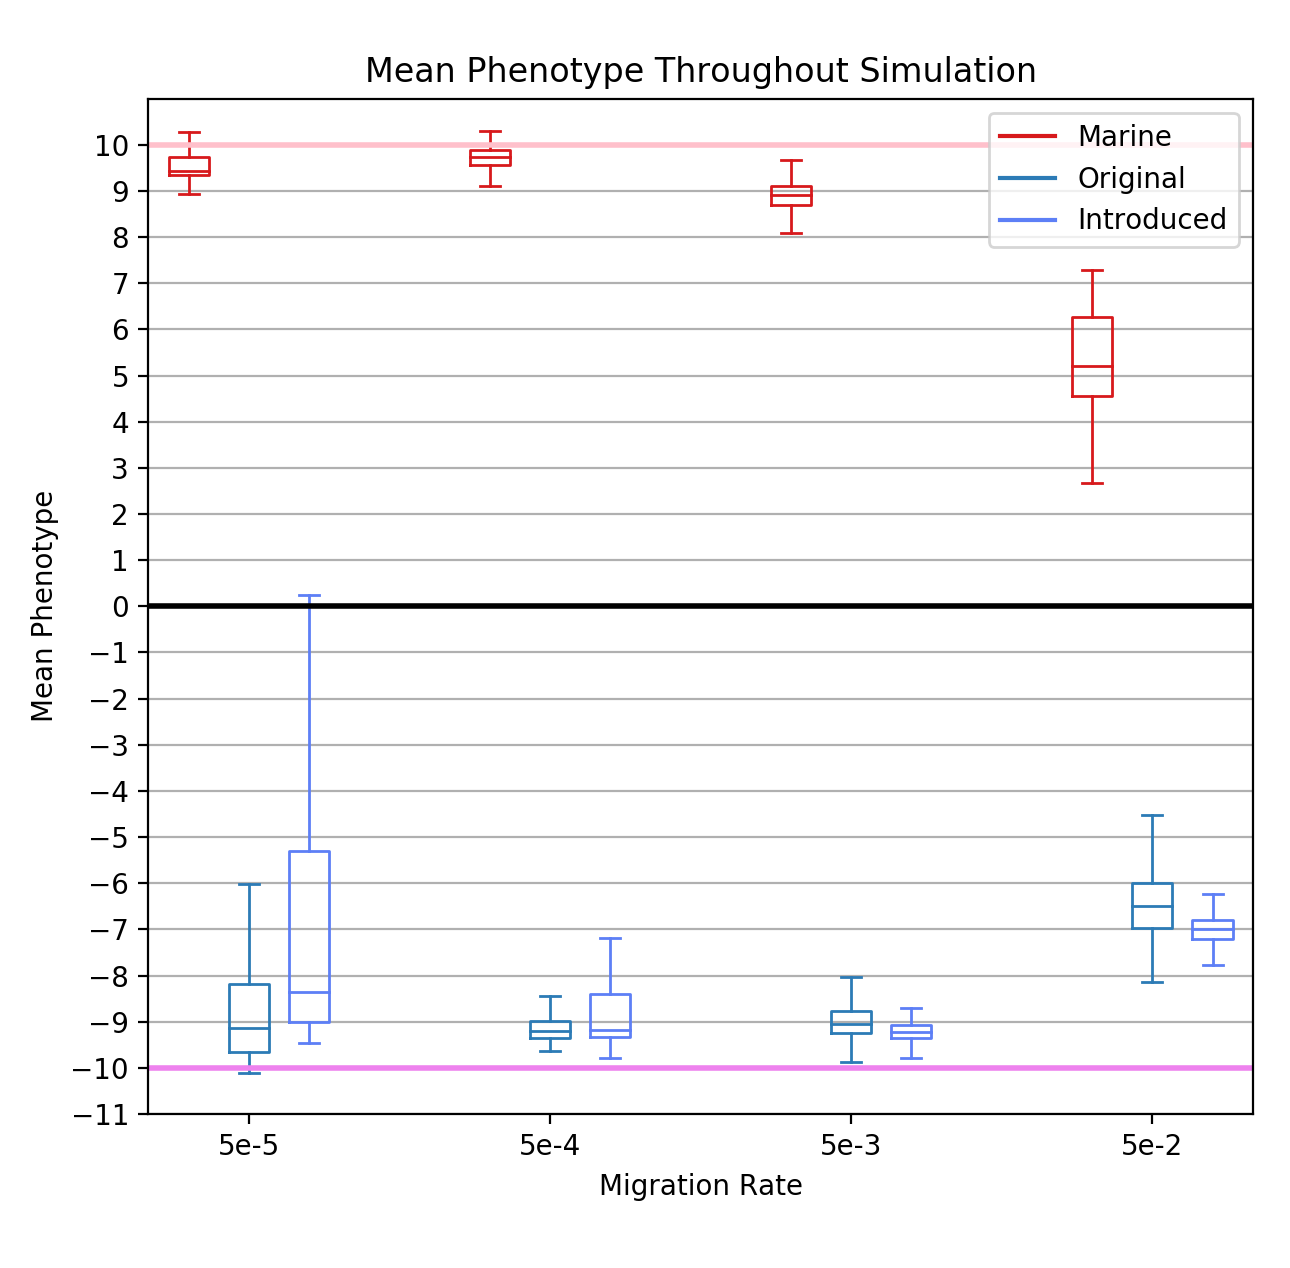
\includegraphics[width=0.6\linewidth]{matplotlibPlots/MeanPhenotype1.png}
  		\caption{
            Distribution of mean trait values throughout each simulation.
            The dashed pink and purple lines show the optima ($\pm 10$).
		}
  		\label{fig:MeanPhenotype}
	\end{center}
\end{figure}
\plr{Is this the whole simulation? what about the initial adaptation phase?
     Is the horizontal line at the median? what are the whiskers at?}


As expected, increasing migration rate decreased differentiation between habitats.
As seen in Figure \ref{fig:Fst},
$F_{ST}$ between marine and freshwater habitats at neutral sites 
steadily declines as migration increases.
Local adaptation was still able to occur despite overall homogenization:
if computed using only sites with alleles affecting the trait (``effect mutations''),
$F_{ST}$ between habitats was relatively constant across migration values.


\begin{figure}
	\begin{center}
  		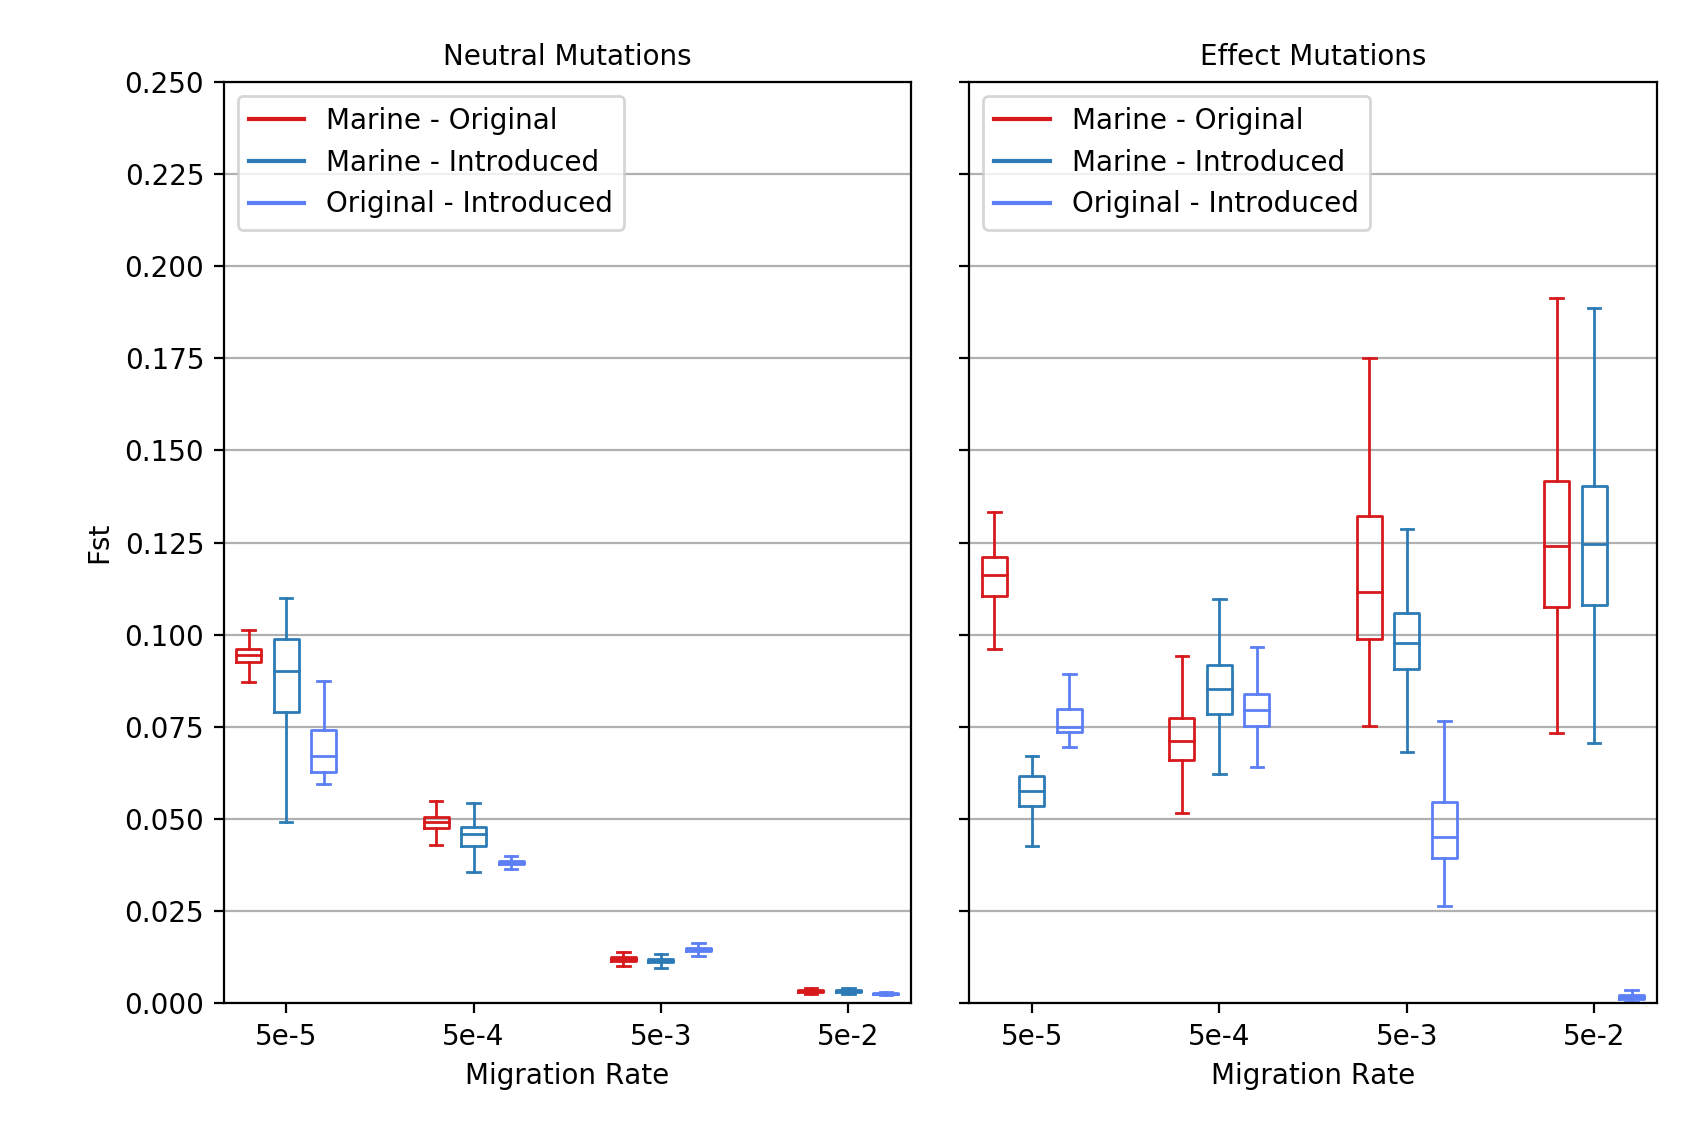
\includegraphics[width=0.8\linewidth]{matplotlibPlots/FST_HRR.png}
  		\caption{
            Distributions of $F_{st}$ values between the three habitats,
            accumulated across the course of the simulation, calculated 
            \textbf{(left)} using only neutral mutations, and
            \textbf{(right)} using effect mutations.
        }
  		\label{fig:Fst}
	\end{center}
\end{figure}


\paragraph*{Speed of adaptation}
Increasing migration rate strongly decreased the time until freshwater habitats could adapt,
both in the initial and introduced sets of lakes.
As shown in Figure \ref{fig:TimeToAdaptation}, at the lowest migration rate 
it took over 20 thousand generations for the mean trait value across introduced lakes to 
get to within 0.5 of the original lakes value.
Although many lakes had adapted before this time,
the different rates of introduction of effect alleles is clearly seen in the traces
of trait values against time (e.g., Figure \ref{fig:phenotype_ts2}).
However, higher migration rates allowed the freshwater habitat to adapt
nearly as quickly as the marine habitat.

\begin{figure}
	\begin{center}
        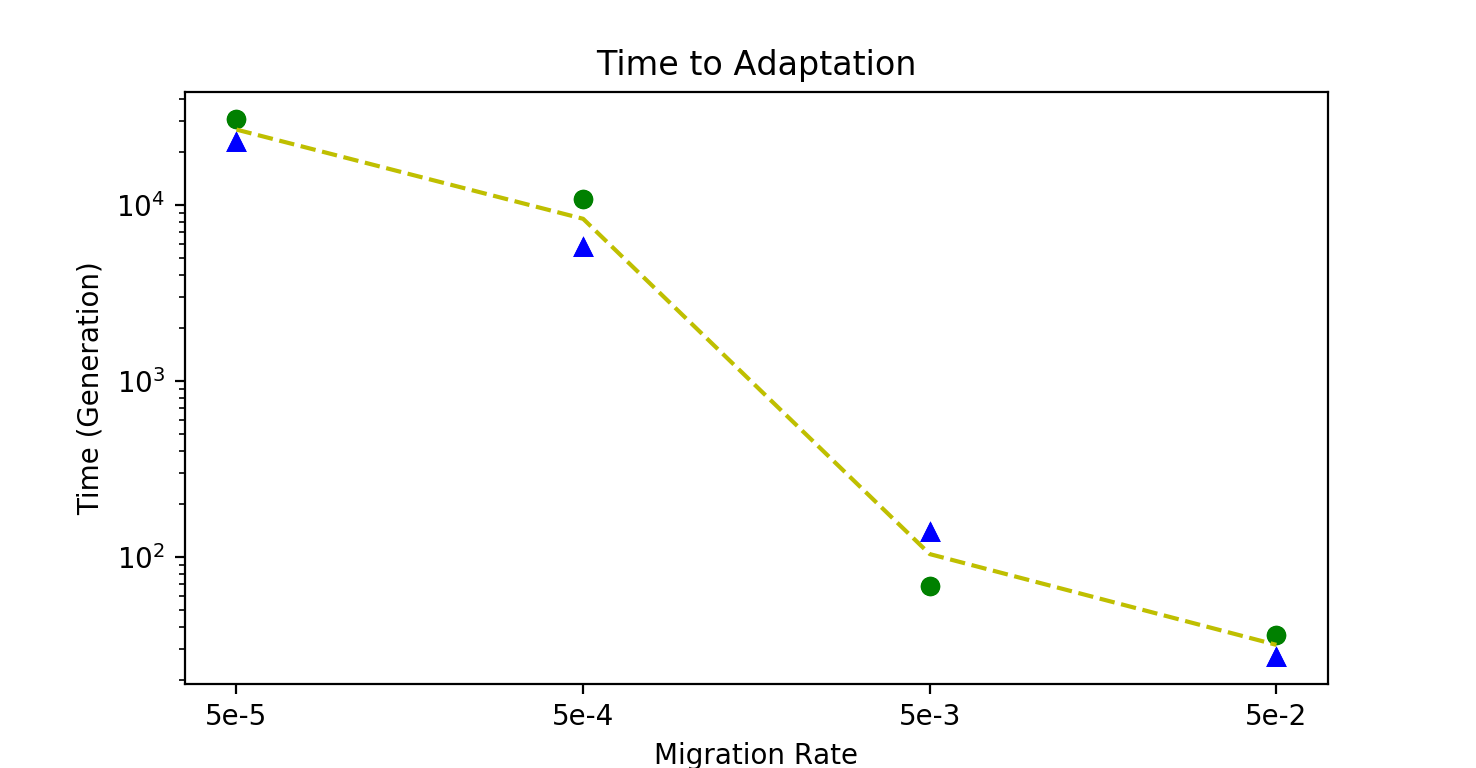
\includegraphics[width=0.8\linewidth]{matplotlibPlots/TimeToAdaptation}
        \caption{
            Time to adaptation as a function of migration rate ($m$),
            measured as the number of generations
            until the introduced population's mean phenotype is within 0.5 
            of the original lakes average phenotype. 
            Each point represents a single simulation, and
            the line shows the average of all points at each value of $m$.
        }
  		\label{fig:TimeToAdaptation}
	\end{center}
\end{figure}


%%%%%%%%%%%%%%%%%%%%%%%%%%%%%%%%%%%%%%%%%%%%%%%%%%%
\subsection*{Sharing of freshwater adapted alleles}

%FIGURES THAT SHOW THIS:
%-MPAA / IND
%-Total/Avg shared

The tenfold difference in speed of adaptation occurs because
at low migration rates, adaptation occurs independently in each lake,
and the marine habitat has ten times the influx of new alleles than any one lake.
In other words, 
greater mixing at higher migration rates allows lakes to share alleles
instead of developing their own genetic basis of adaptation.
As a first indication of this, Figure \ref{fig:Fst} shows that
$F_{ST}$ between the ``original'' and ``introduced'' sets of lakes 
at effect mutations decreased with migration rate.

To further investigate sharing of locally adaptive alleles
and the transporter hypothesis,
we investigate the ``pre-existing freshwater adapted alleles'',
defined for a particular generation
to be effect mutations above 50\% in at least one original lake and below 50\% in the marine habitat
in that generation.
Figure \ref{fig:MPFAI}A shows the distribution of the number of these alleles,
across generations,
as well as the average number of lakes each is found in.
As migration rates increase, the number of these alleles decreases steadily,
and each is concurrently found in a greater number of lakes.

As the number of common, locally adaptive alleles decreases,
the genetic basis of adaptation is more commonly shared.
Figure \ref{fig:MPFAI}B shows
the distribution of the mean percentage of currently-defined freshwater adapted alleles 
that each genome in each of the populations carries,
averaged across time and individuals.
If all individuals across lakes carried the same set of alleles determining their trait value,
this would be 100\%.
This value is nearly reached at the highest migration rate;
but it is lower due to migration load.
At the lowest migration rate, 
each genome in the original lakes have almost exactly $1/10^{th}$ 
of the total freshwater adapted alleles --
since there are 10 lakes, this implies that each lake has adapted with a unique set of alleles.
Since these are \emph{pre-existing} alleles, the value is zero for introduced lakes.


\begin{figure}
	\begin{center}
        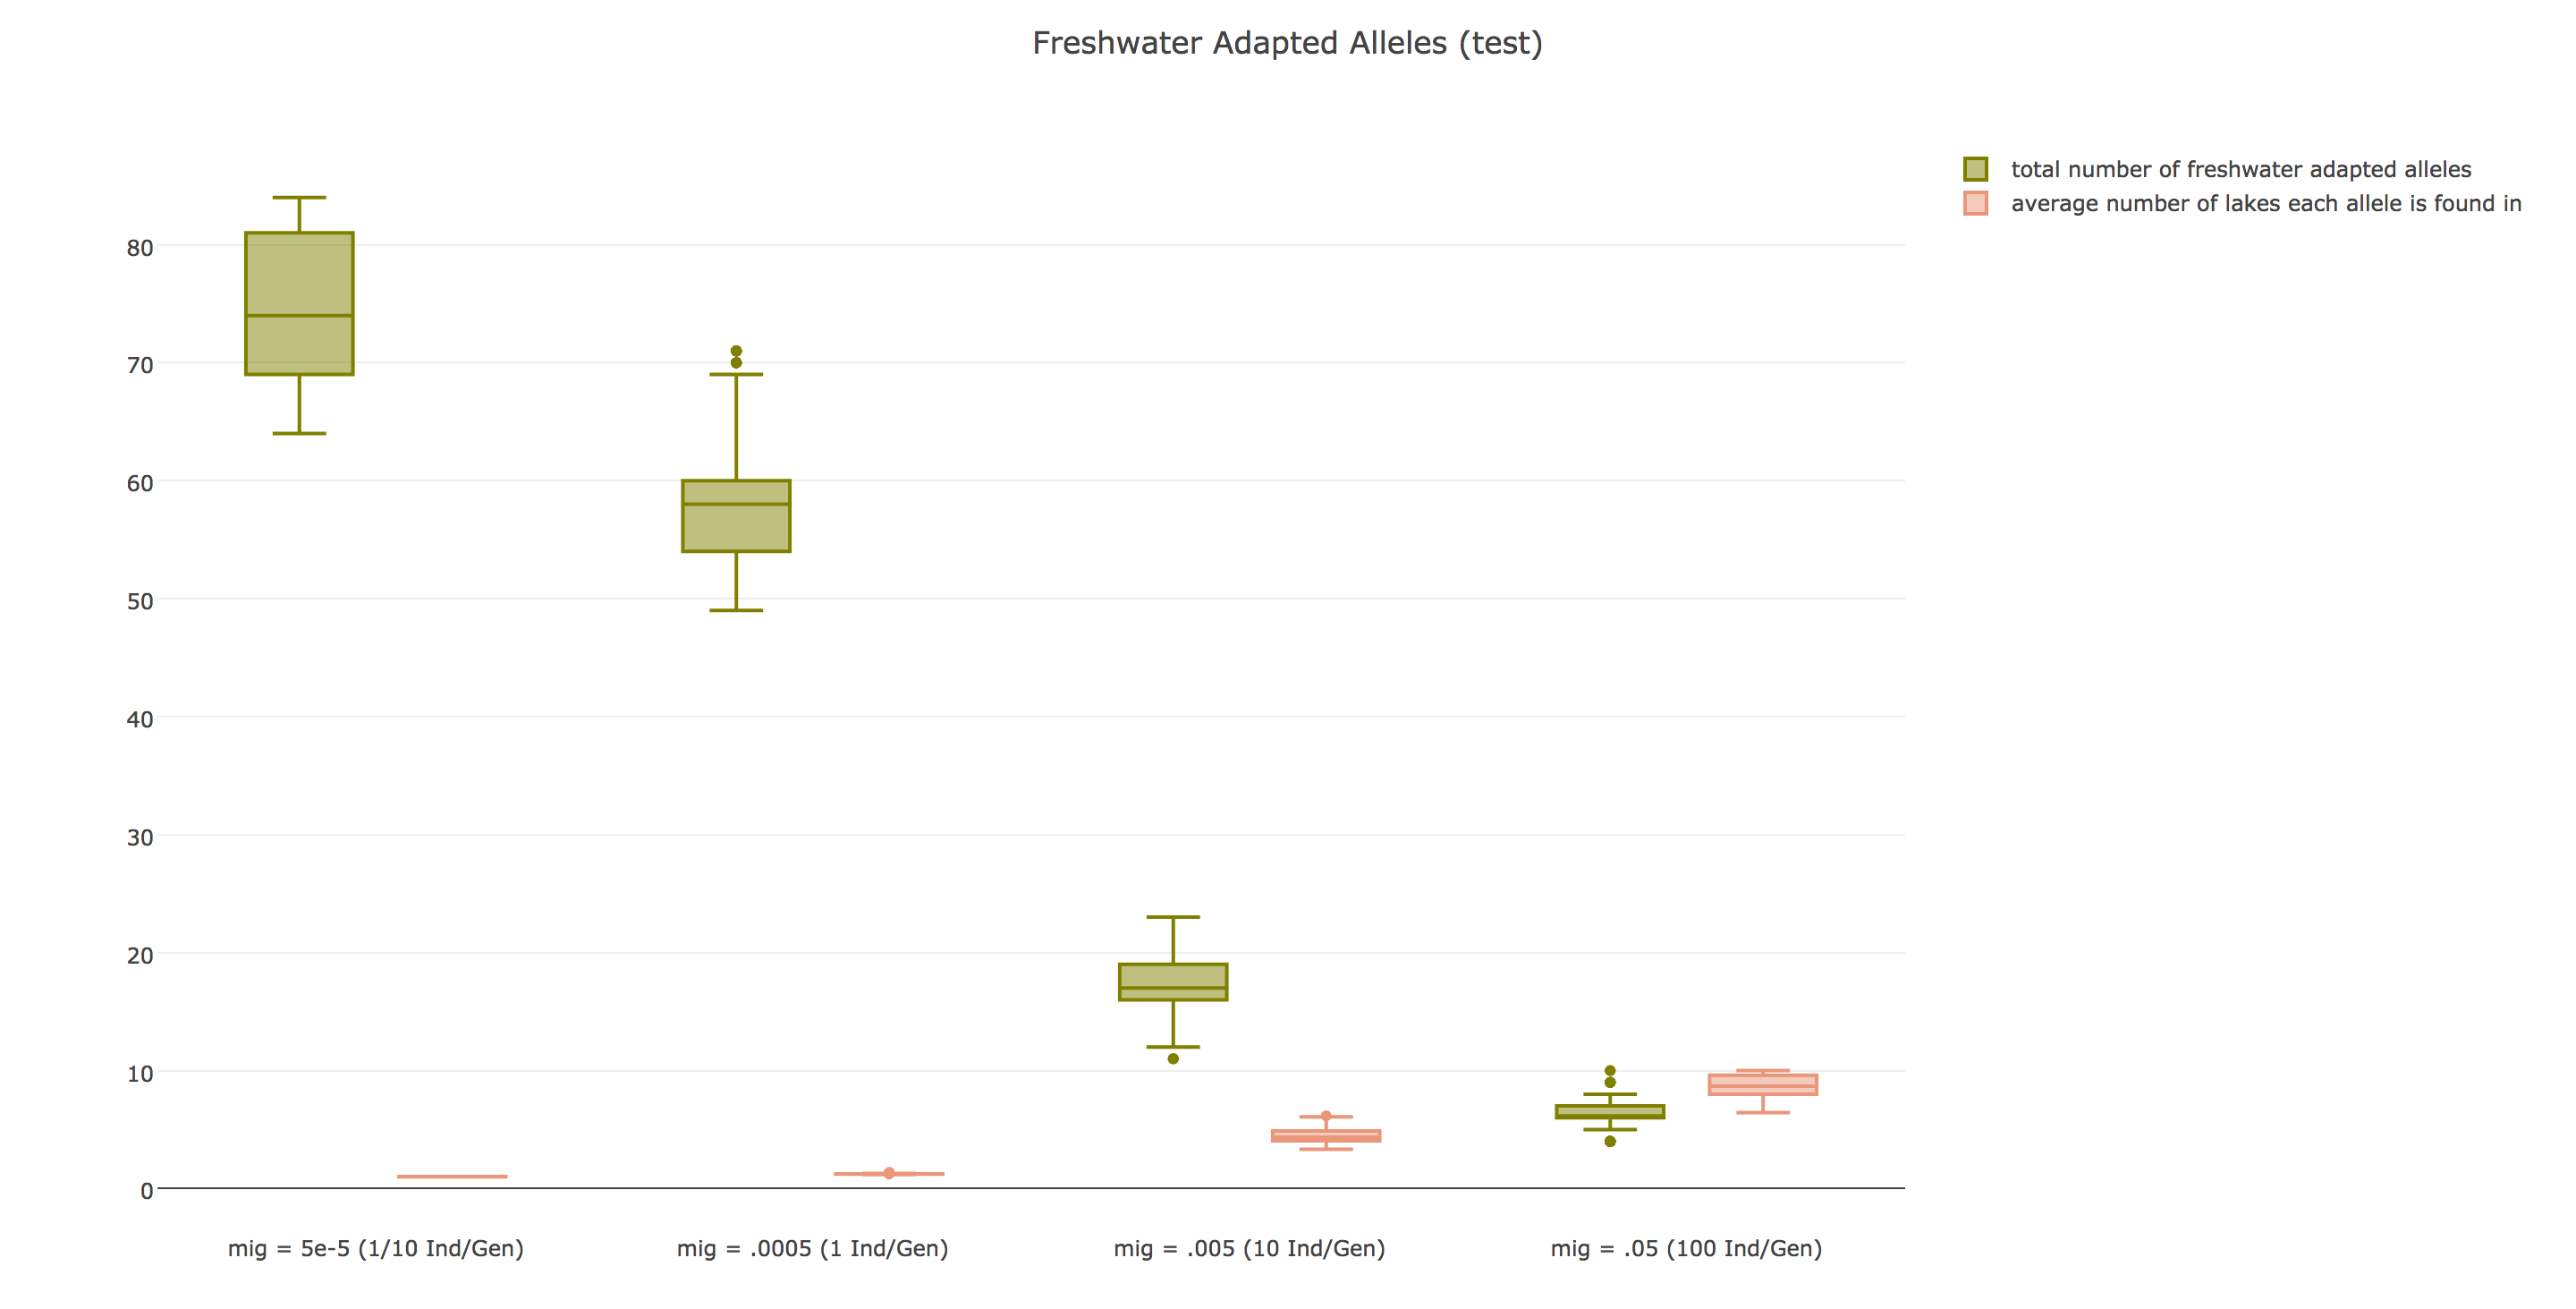
\includegraphics[width=\linewidth]{plotlyPlots/NumFAA}
        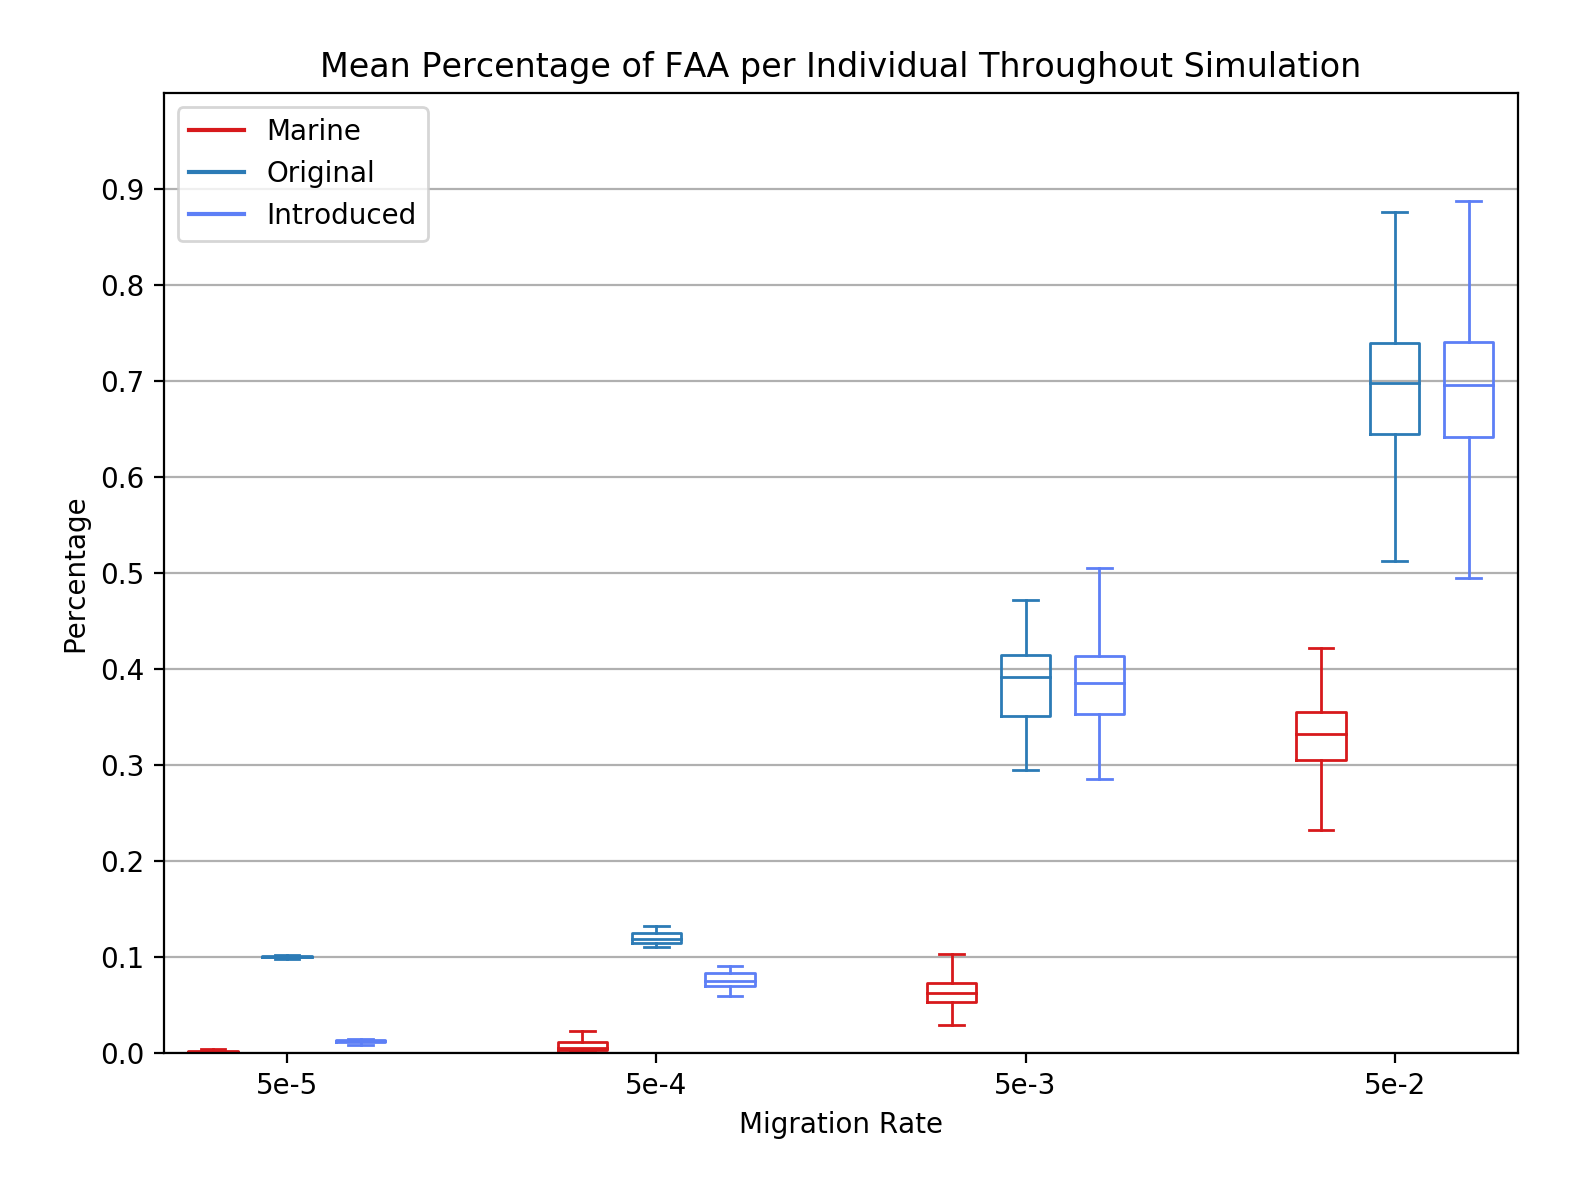
\includegraphics[width=\linewidth]{matplotlibPlots/MPFAI}
  		\caption{
            \textbf{(A)}
            Distribution of the number of freshwater adapted alleles (green)
            and the average number of lakes each allele is present in (red)
            across the course of the simulation.
            \textbf{(B)}
            Distributions of mean percentage of freshwater adapted alleles (FAA) per individual throughout the simulation run, for each subpopulation.
		We count the total number of freshwater alleles for each individual before averaging them in each population and dividing by the total number of defined
		freshwater adapted alleles.
		Looking at total number of FAA per individual gives us an idea behind how many alleles underly a freshwater haplotype, 
		while the percentage tells us the variance of the haplotype}
		\label{fig:MPFAI}
	\end{center}
\end{figure}



%%%%%%%%%%%%%%%%%%%%%%%%%%%%
\subsection*{Migration load and genetic variation}

%FIGURES THAT SHOW THIS:
%- Phenotype Distribution
%GENERAL

At first, increased migration allows sharing of adaptive alleles between lakes,
but at the highest migration rate,
the constant influx of alleles between the habitats creates substantial migration load.
This rate, $m=.05$, only replaces 5\% of each population each generation
with migrants from the other habitat, but this is sufficient to shift the mean trait values
to nearly half their optimal values, as seen in Figure \ref{fig:MeanPhenotype}.
Significant gene flow constricts local adaptation
as a consequence of a large number of offspring through hybridization events between subpopulations.

\paragraph{Standing genetic variation}
Despite a dramatic difference in the amount of allelic sharing between lakes,
standing genetic variance (Figure \ref{fig:SGV}) was around 0.05 in the freshwater habitat
across all but the highest migration rates.
Concurrently,
genetic variation in the marine population steady increased with migration
to a similar value.
On the one hand, it is not surprising that lakes, as a group,
carry more genetic variation than the marine habitat,
since population subdivision allows different alleles to become common in each.
However, it is striking that at $m=.005$, the marine habitat carries as much genetic variation,
despite a lack of any substantial migration load.



%%%%%%%%%%%%%%%%%%%%%%%%%%%%%%%%%%%%%%%%%%%
\subsection*{Realized genomic architecture}


\begin{figure}
	\begin{center}
        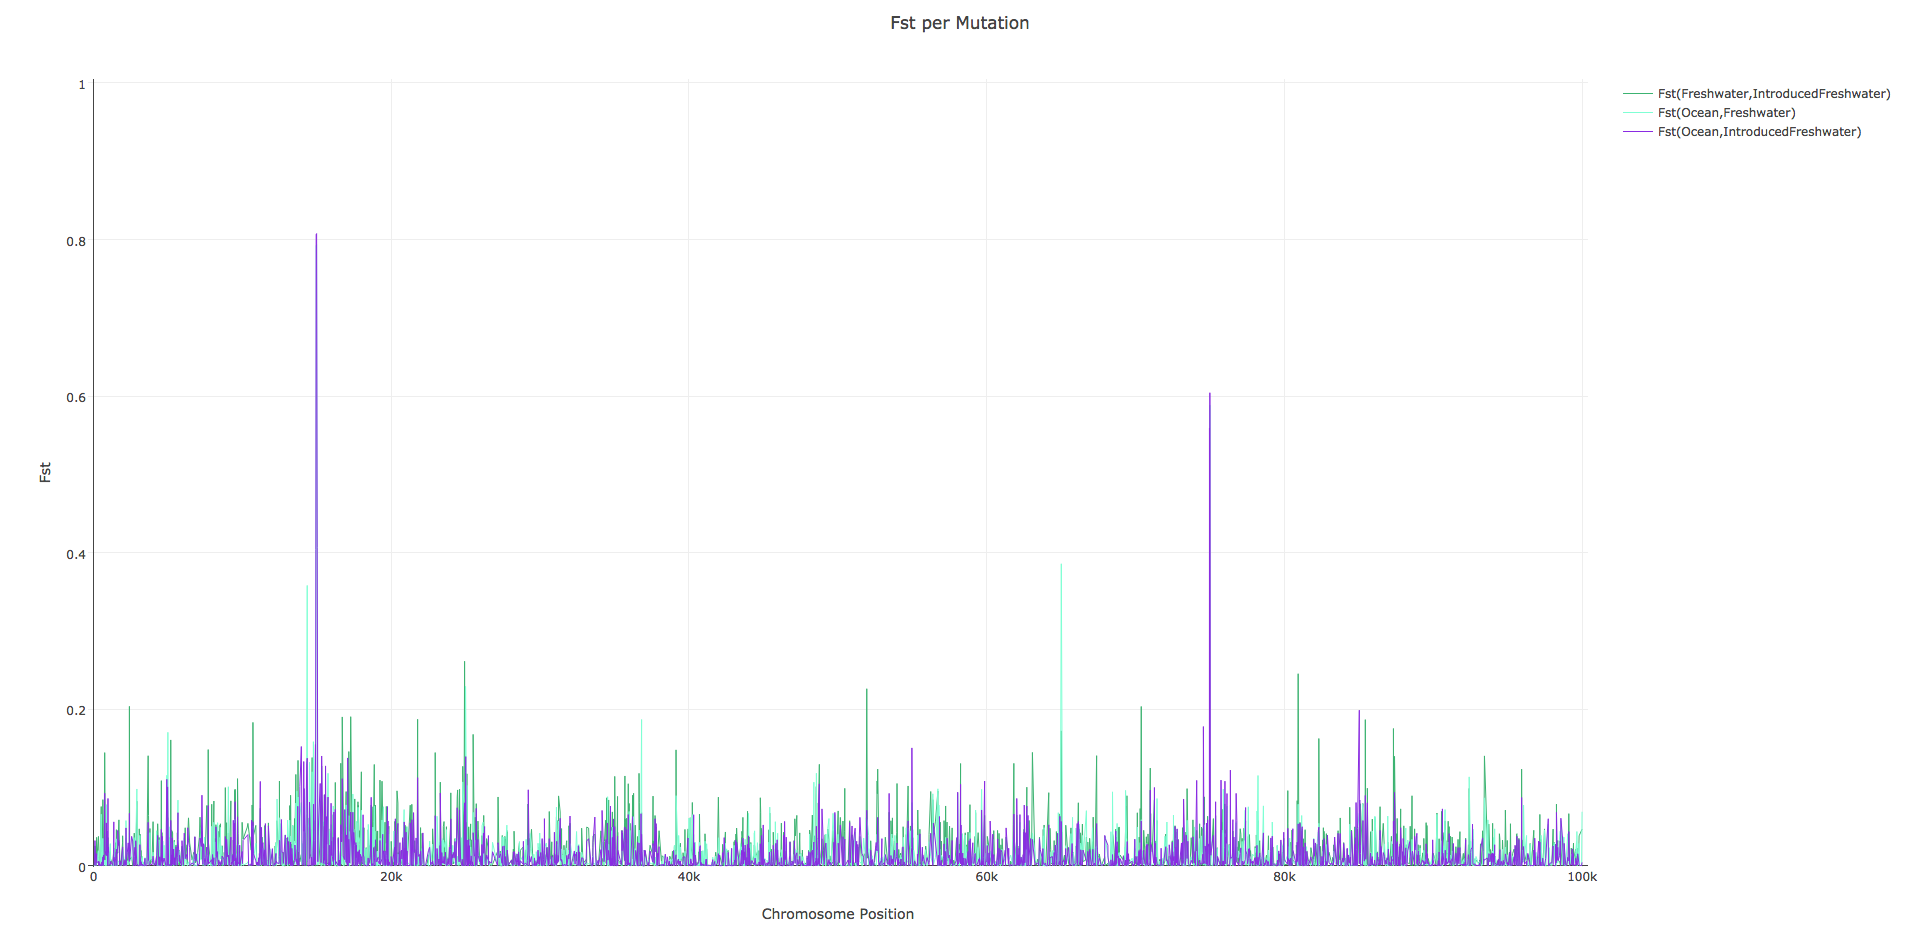
\includegraphics[width=0.7\linewidth]{plotlyPlots/FstAcross5e-3}
        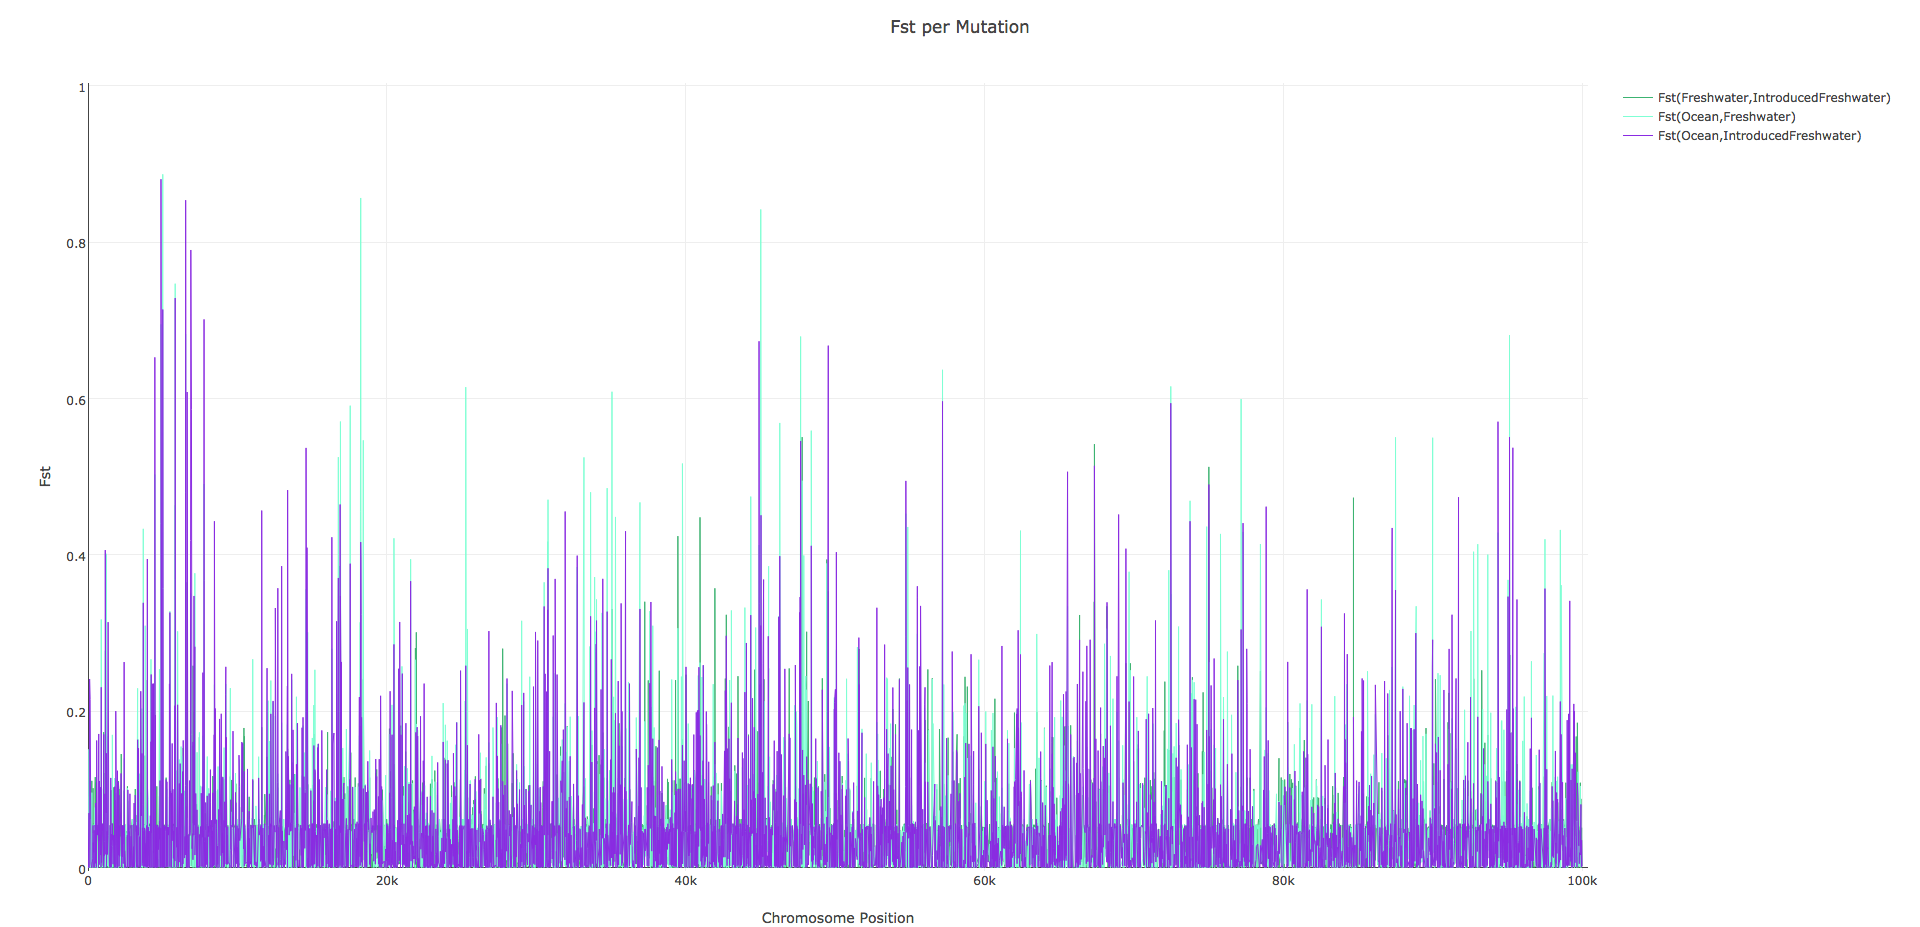
\includegraphics[width=0.7\linewidth]{plotlyPlots/FstAcross5e-4}
  		\caption{(Description and cleaning needed)
		}
  		\label{fig:Fst3}
	\end{center}
\end{figure}

Now we take a closer look at the genomic architecture of local adaptation 
between the two habitats.
Do the alleles underlying trait differences cluster along the genome?
Do measures of local differentiation identify the causal loci?
Figure \ref{fig:Fst3} shows plots along the genome of per-locus $F_{ST}$ values
between the marine and original freshwater habitats
at the two intermediate migration rates.
(Note that we are pooling freshwater habitats; 
a single lake would provide substantially less power.)

\plr{need to know where the FAA are in these figures}

Higher migration rates showed more distinct $F_{ST}$ peaks
over polymorphic loci underlying trait differences between the habitats.
As migration rate decreased, the ``background'' levels of $F_{ST}$ increased,
swamping out this signal until the regions under selection were indistinguishable. 
This is likely due to two reasons: 
first, stronger genetic drift with less migration leading to higher background $F_{ST}$,
and second, greater sharing of adaptive alleles providing a shared signal across populations.

This suggests that genome scans for local adaptation
based purely on measures of differentiation
will only be successful given enough migration between habitats.
To quantify this, Figure \ref{fig:Power_FP} shows the power and false positive rates
that would be obtained by an $F_{ST}$ cutoff that declared everything above a certain value
to be a causal locus.
\plr{Labels are wrong on that figure: false pos rate should go down with cutoff.
     Is it true positive rate?}

\begin{figure}
	\begin{center}
  		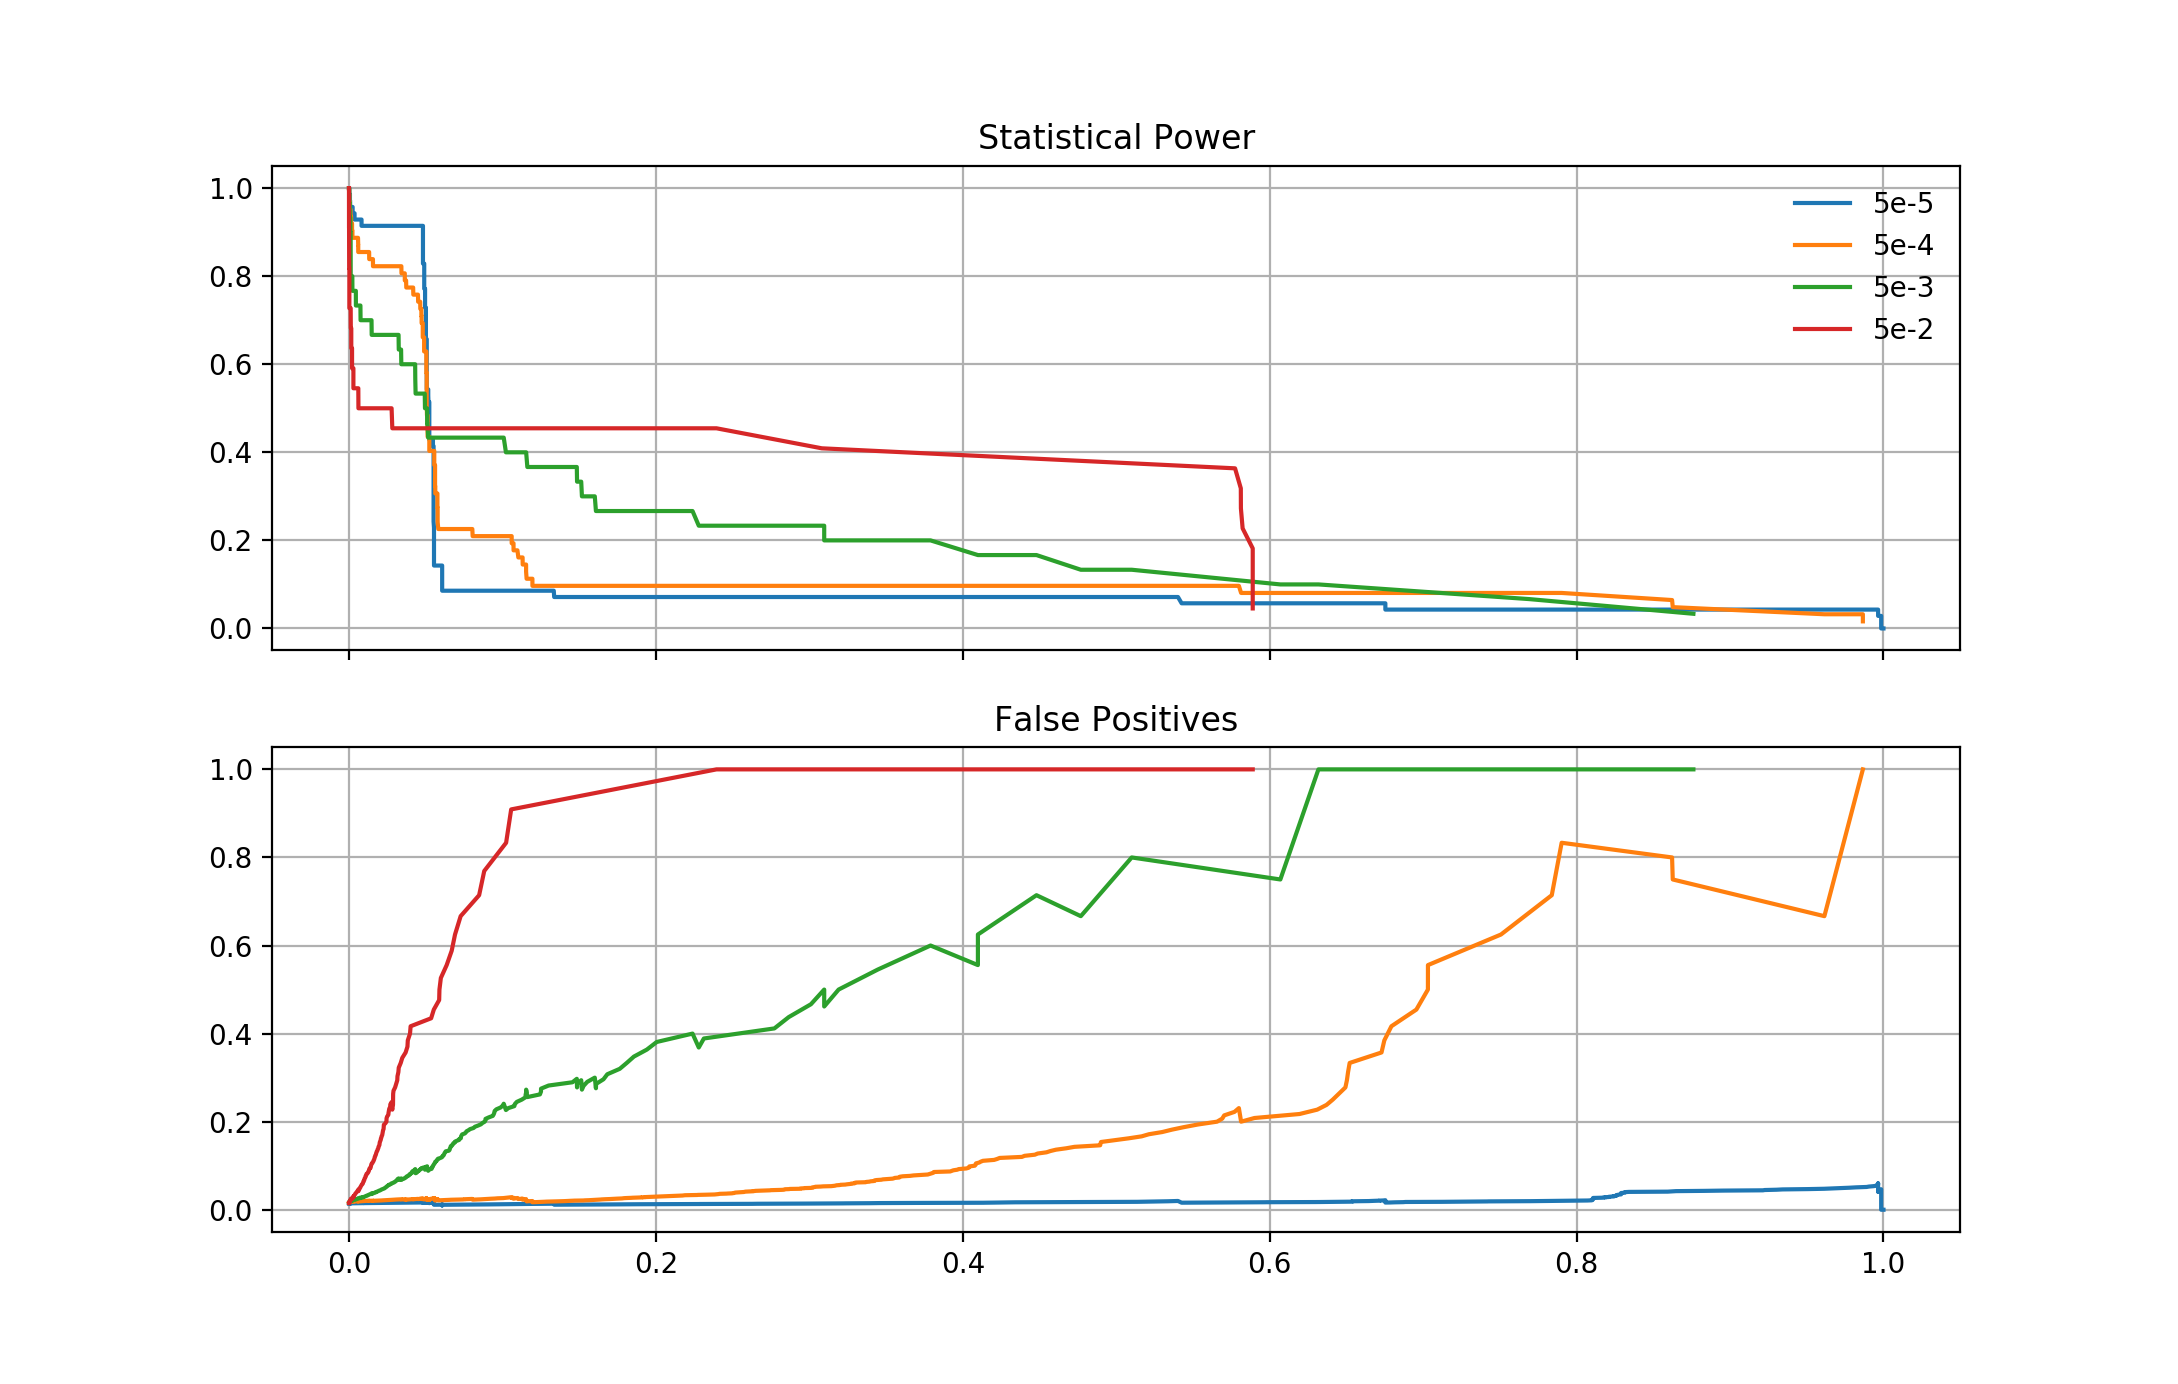
\includegraphics[width=0.7\linewidth]{matplotlibPlots/Power_FP.png}
  		\caption{ 
		%SP - suppose you have an Fst Peak, how likely is it that that region is causal. 
		Statistical Power and False Positives as a function of $F_{st}$ threshold. 
		Statistical Power is the likelihood that a SNP will be predicted to have an effect on phenotype when there is an effect to be detected (?).
		False Positives give us the ratio of SNPs that effect phenotype to total SNPs greater than the $F_{st}$ threshold.
        TODO: x-axis label ($F_{ST}$).
		}
  		\label{fig:Power_FP}
	\end{center}
\end{figure}

With 10 effect regions across the genome, we can see in \ref{fig:Fst3} that only about 1 or 2 of the region contain peaks. 
%SOFT STATEMENT - MORE (Peak) EVALUATION?
When looking closely at the peaks we see that each is usually a composition of 7-8 SNPs close in proximity.
%SOFT STATEMENT -
Because some of those mutations are selectively neutral (we can see this because the counts of FAA are not as high as the number in the clusters),
this is suggestive of hitchhiking alleles along with the SNPs being brought to high frequency by a selective sweeps.


In regions of the genome underlying individual trait value, we observed 
Given that migration increases the gene flow between subpopulations, how valid are $F_{st}$ peaks at different $M$. 
Knowing exactly which mutations effect phenotype in our simulations, 
we can look at the statistical power and false positives given $F_{st}$ per SNP across the genome. 
In Figure \ref{fig:Power_FP} , looking at an $F_{st}$ threshold greater than 1, we see the two lowest migration rates $10^{-5}$ and $10^{-4}$ having very little statical power. 
This along with low false positive rate across all $F_{st}$ threshold values is fairly predictable when you consider the high $F_{st}$ values across the genome. 

%The lowest migration rate of $10^{-5}$ also has a very low false positive rate across all $F_{st}$ threshold values.
%\subsubsection*{Low Recombination Causes Clustering}


%%%%%%%%%%%%%%%%%%%%%%%%%%%%%%%%%%%%%%
\subsection*{Theoretical expectations}
\plr{does this go first or second?}

Here's some rough calculations to get a sense for what should be going on.
Everything is done in more detail in OTHER PLACES WE SHOULD CITE.
Fisher, Chevin, etc.

Suppose a new allele enters a lake, either by migration or mutation.
If, when it is rare but present in $n$ copies,
it has fitness advantage $s$
-- i.e., the expected number of copies in the next generation is $(1+s)n$ --
then the probability that it escapes demographic stochasticity to become common in the population
is approximately $2s$ \citep{fisher,prob_fixation}.
If the current population all differed from the optimum trait by $z$,
and the allele has effect size $-u$ in heterozygotes,
then the fitness advantage of the allele would be
$s(u) = \exp(-\beta((z - u)^2) / \exp( - \beta z^2)) \approx 2 \beta z u$,
where in our parameterization, $\beta = 1 / 450$.
This tells us two things:
(1) the rate of adaptation decreases as the population approaches the optimum,
and (2) larger mutations (in the right direction) are more likely to fix.

\paragraph{New mutations}
The total rate of appearance of new mutations per lake is $\mu_L = 0.04$,
which are divided evenly in seven categories: neutral, and then additive, dominant, and recessive
in either direction.
This implies that a new additive or dominant effect mutation appears once every 87.5 generations,
on average.
Effect sizes are Exponential with mean $1/2$, and as above the probability
and so the probability that a dominant mutation manages to establish in a population differing from
the optimum by $z$ is roughly
$\int_0^\infty 4 \beta z u \exp(-2u) du = \beta z$,
and so the rate of establishment of dominant mutations is $\beta z / 87.5$,
i.e., about one such mutation every $2461/z$ generations.
The distribution of these successfully established mutations 
has density proportional to $u \exp(-2u)$, i.e., is Gamma with mean 1 and shape parameter 2.
Since additive alleles have half the effect in heterozygotes,
they have half the probability of establishment.
Combining these, we expect during the initial phase of adaptation,
when the populations begin at around distance $z=10$ from the optimum,
adaptive alleles to appear through mutation on a time scale of 250 generations,
and each to move the trait by a distance of order 1.

\paragraph{Migration}
A allele that moves the trait $z=1$ units in the freshwater direction
has fitness roughly $\exp(-\beta) \approx 1 - \beta$ in the marine environment
(which is close to optimal).
The product of population size and fitness differential in the marine environment
is therefore $2Ns = 8.9$, implying that these alleles are strongly selected against
but might occasionally drift to moderate frequency.

TODO: estimate rate at which migrant alleles move between lakes



%%%%%%%%%%%%%%%%%%%%
\section{Discussion}

We have shown that historical introgression, at our given parameter sets,
is able to reproduce rapid and parallel adaptation similar to what we've seen in real populations such as Middleton island.
Selection is able to rebuild the freshwater haplotype from marine populations as a medium between all freshwater populations.
Almost all rates of migration were helpful in the efficiency of the population to locally adapt except for the highest at which migration load 
limited the ability of the populations to reach the local optimum. 

We also have also explored the genomic architecture as a consequence of the nature of selection in our scenario. 
The alleles underlying individual trait value were of large effect and a low number. 
With a total of $10^{5}$ loci, to be realistic, each loci should represent 1000 $Kb$ in real data.
\jgg{This should be expanded upon, not sure what this means in terms of the genomic architecture}

We have also shown introgression is beneficial for inferring causative loci from divergence ($F_{st}$) along the genome. 
This is generally because noise of selectively neutral alleles divergence can appear causative when genetic drift causes more 
differences between populations that have little gene flow between them.
It's important to know that in all scenarios, hitchhiking of selectively neutral alleles could also be 
mistaken for being causative as they often display the same amount of divergence.
%wouldn't it be cool if we could use this fact and simulate introgression, starting with real data that is noisy to extrapolate the areas we care about?
%this could be nonsense 

% at low M we should be able to predict something ---
% at high M we should be able to predict something ----

%Here, we suggest a range of migration rate (introgression) parameter values which would allow for the rapid (and in turn, parallel) adaptation 
%of marine stickleback introduced intro a freshwater environment.
%While this range is heavily effected by all other selections of parameter values. 

%(1) There's a threshold of introgression for both rapid adaptation and migration load. 
%(1.5) Maybe refer to the literature for migration load.  
\subsection*{thresholds}

We have found that too little migration leads to selection upon new mutations in all subpopulations and lakes alike. 
In contrast, at high migration rates we have seen that migration load limits 
the ability for species to locally adapt to the selective pressure of their environment.
This leads us to consider a window of introgression which allows for the transportation
of FAA's without migration load. 


\subsection*{connect results back to real data?}

%In a species that commonly is subjected to two general types of selective pressure 
%such as marine and freshwater stickleback this is suggestive of the benefit of hybridization in all subpopulations before
%reaching a point of pre or post zygotic 

%(3) discuss what signals researchers could possibly look out for or connect to real data

\paragraph{The adaptive filter?}
RAMBLING THOUGHTS HERE
Since larger effect alleles are more likely to establish,
be it by mutation or migration,
repeated colonization of new freshwater habitats will select for larger alleles,
be it single alleles or haplotypes bound together by an inversion.
However, these are more strongly selected against in the interstitial time.
Being recessive would help with this,
but would also make it more difficult to establish.

\bibliographystyle{plainnat}
\bibliography{Citations}{}

%%%%%%%%%%%%%%%%%%%%%%%%%
\clearpage
\appendix
\section{Supp.}

\begin{figure}
	\begin{center}
  		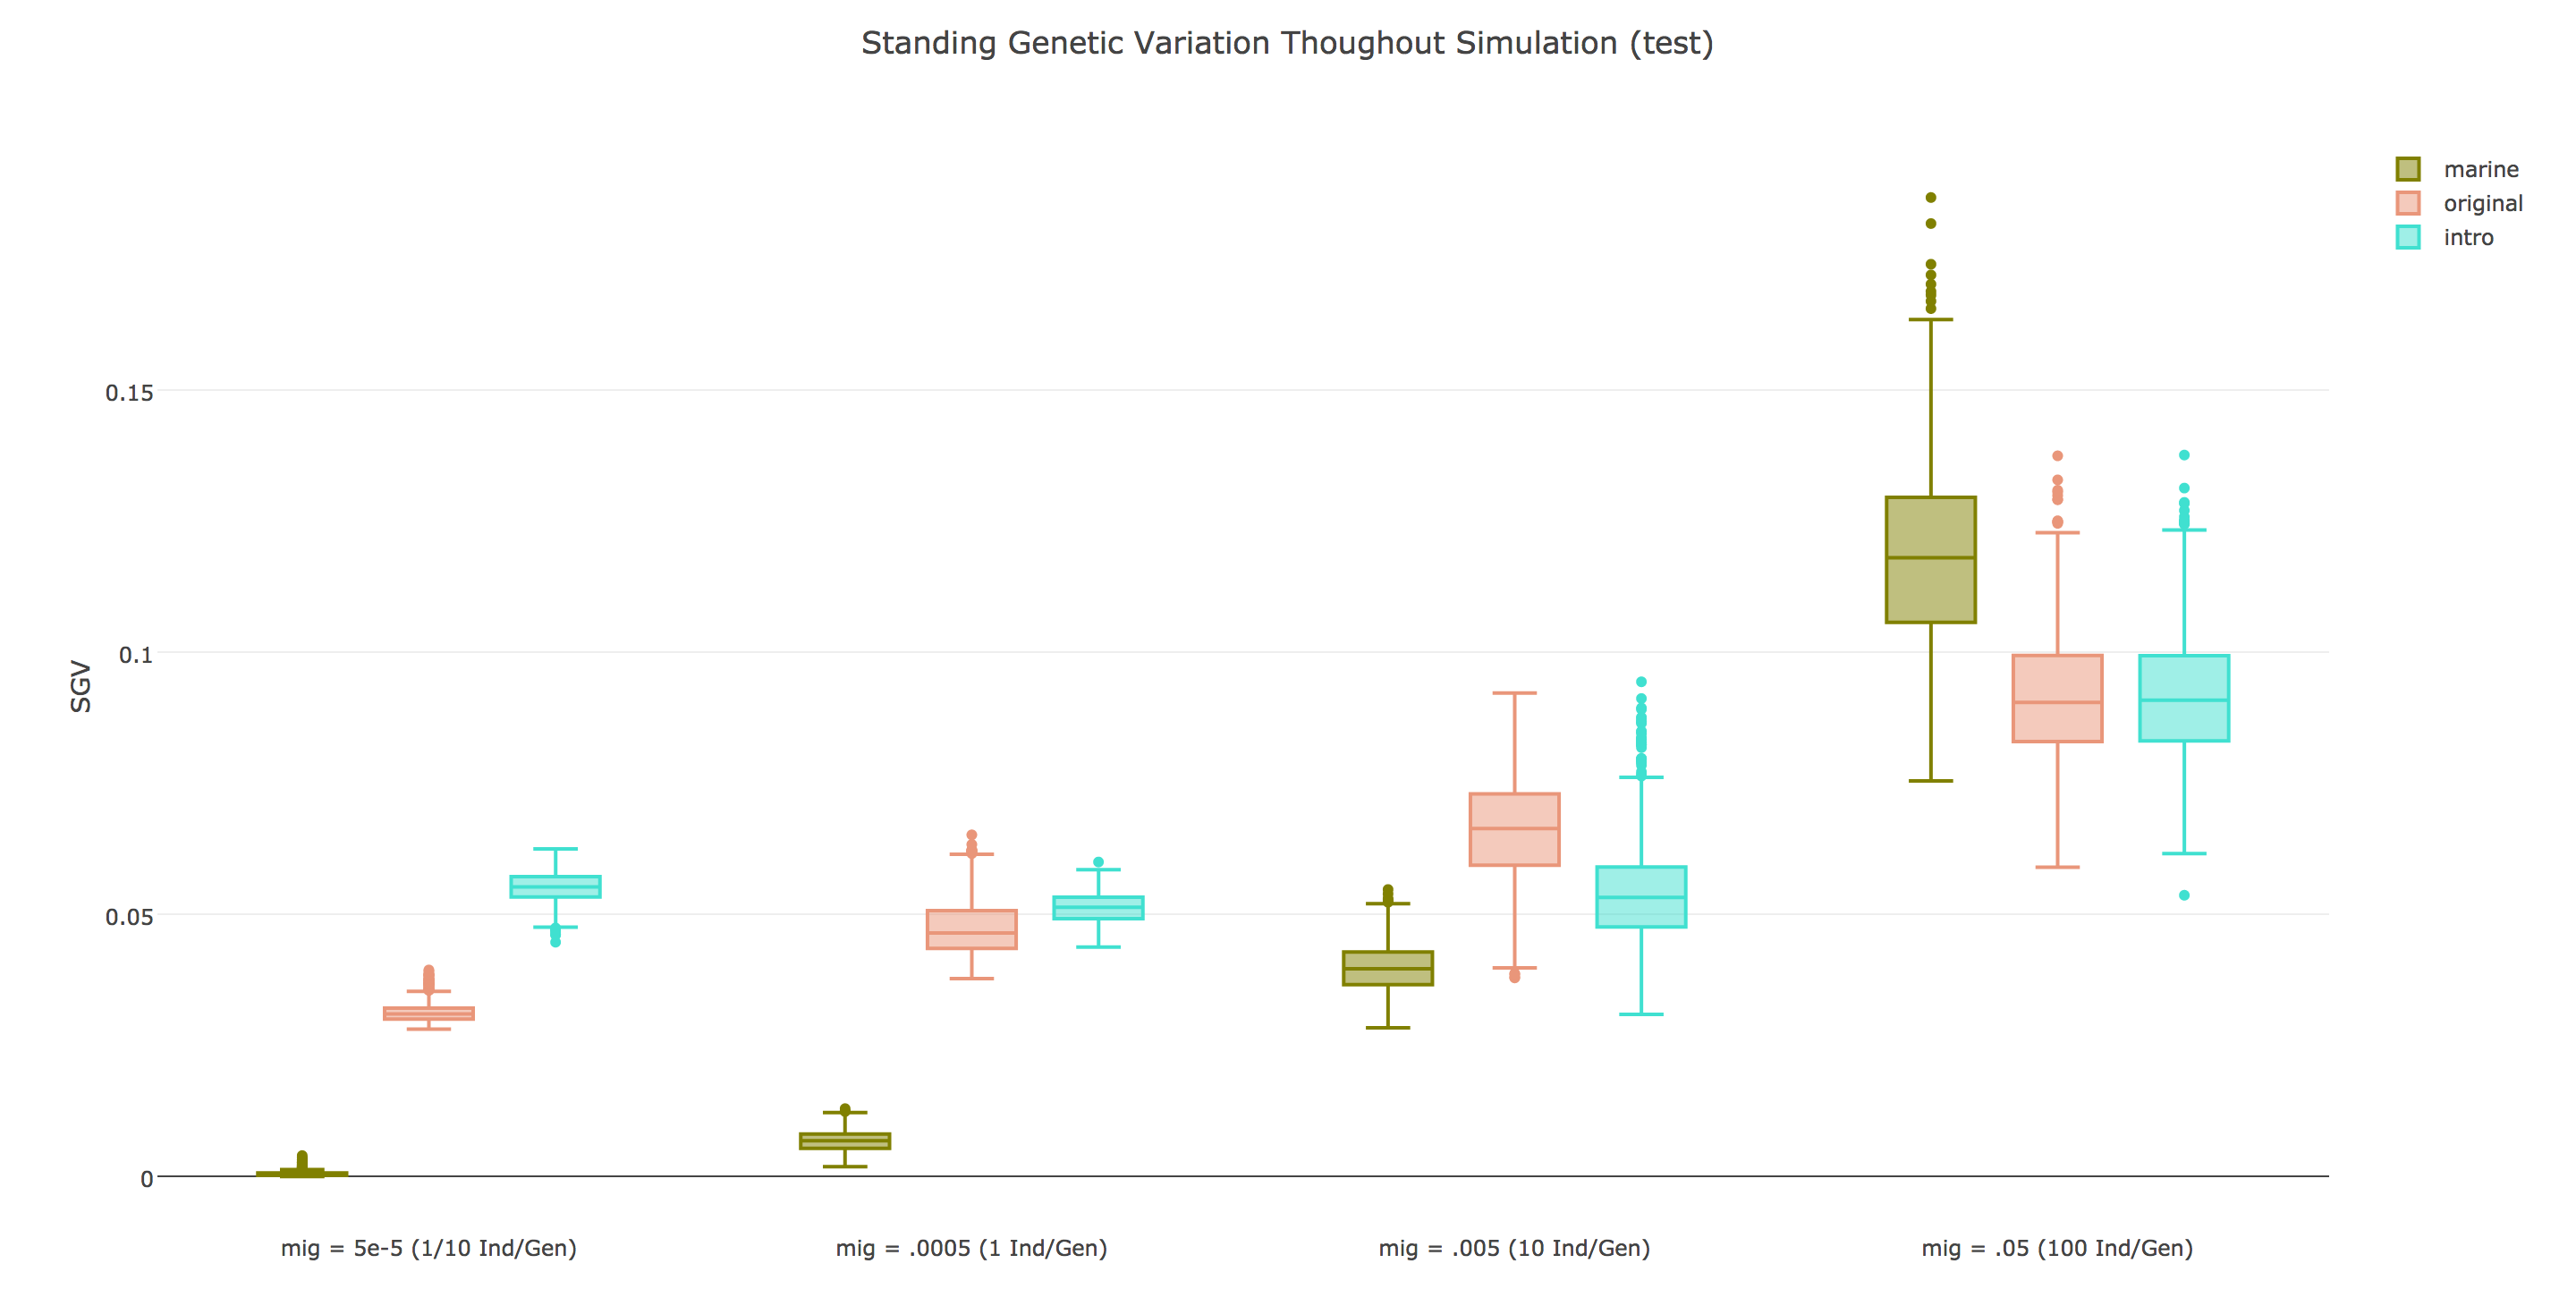
\includegraphics[width=\linewidth]{plotlyPlots/StandingGeneticVariation.png}
  		\caption{(PLACEHOLDER)}
		\label{fig:SGV}
	\end{center}
\end{figure}

\begin{figure}
	\begin{center}
  		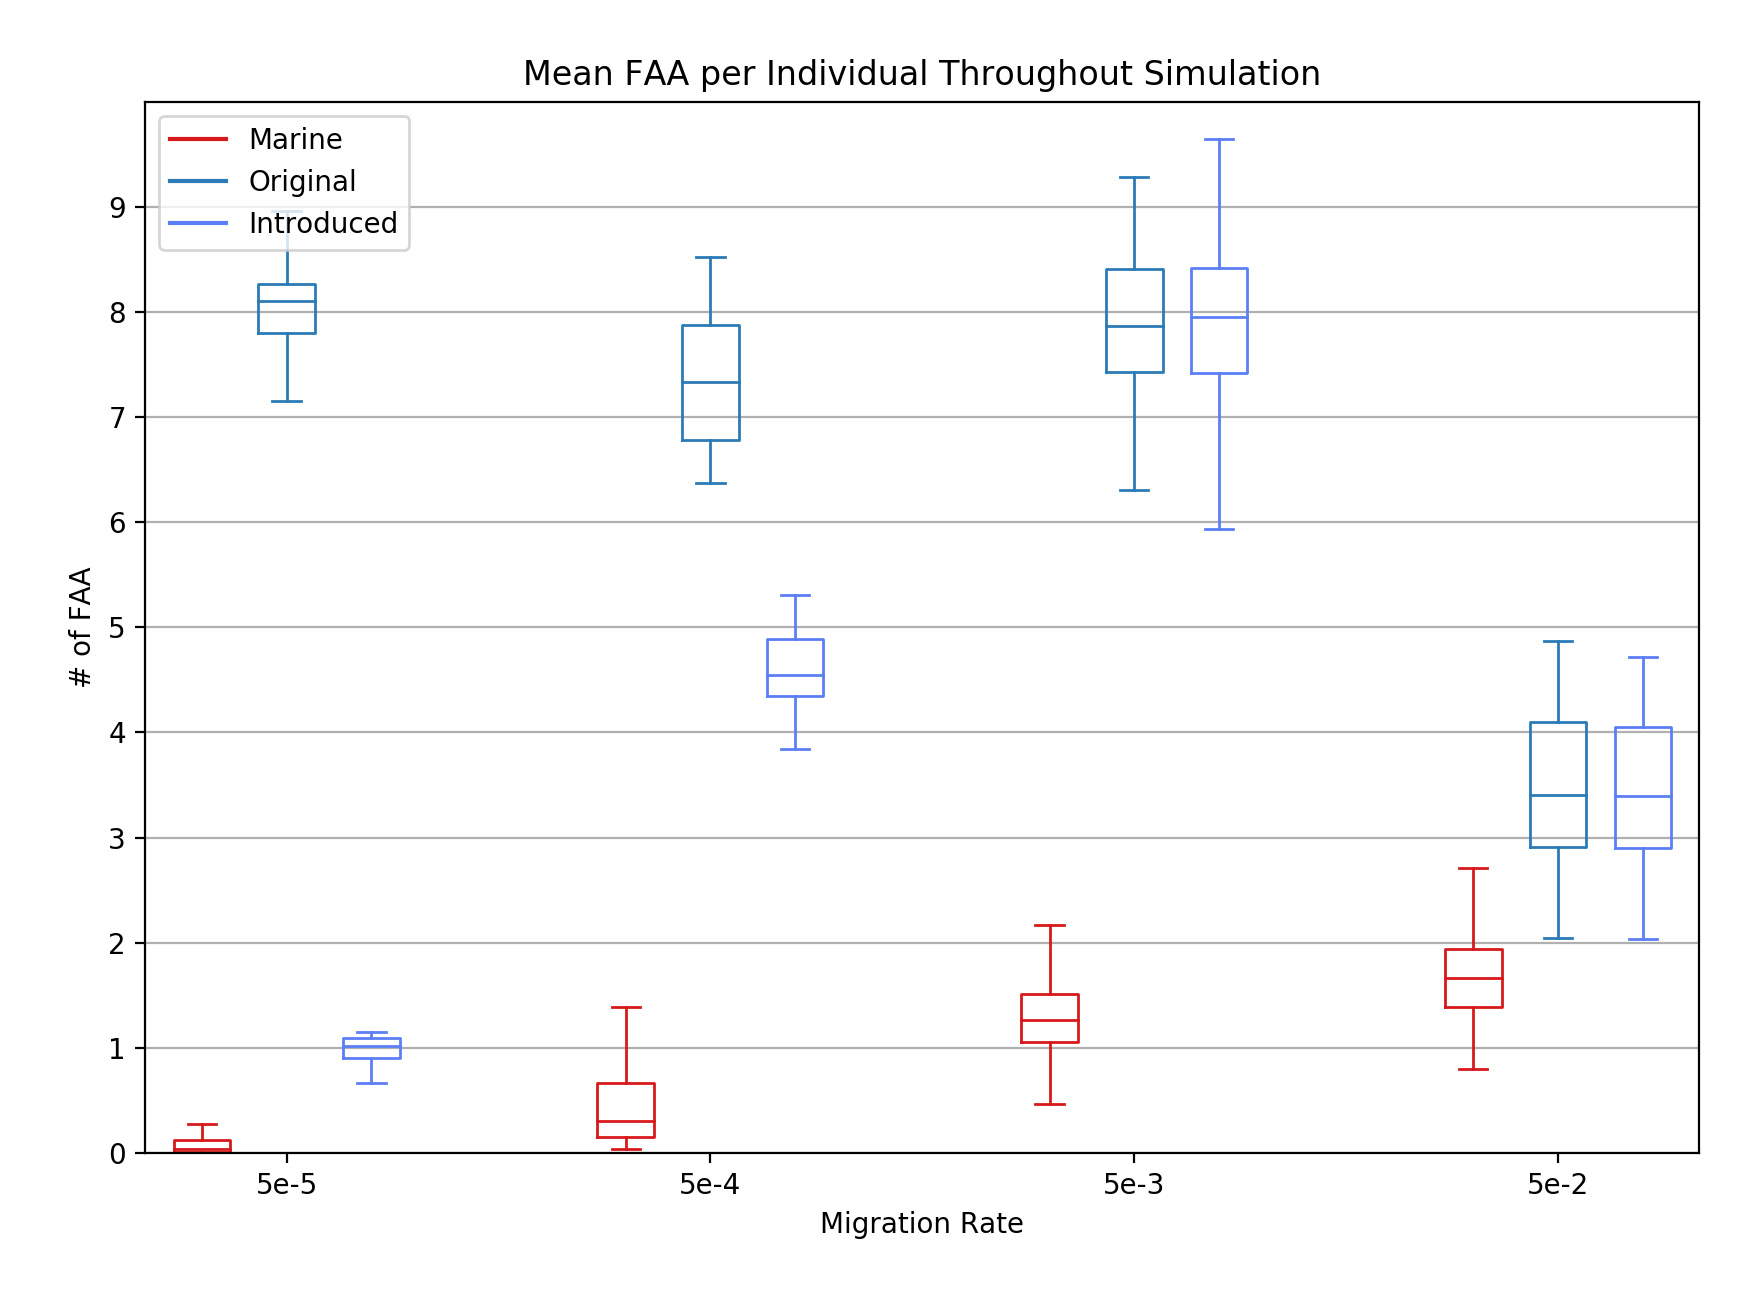
\includegraphics[width=\linewidth]{matplotlibPlots/MFAI.png}
  		\caption{Distributions of mean number of freshwater adapted alleles (FAA) per individual throughout the simulation run, for each subpopulation.
		We count the total number of freshwater alleles for each individual before averaging them in each population and dividing by the total number of defined
		freshwater adapted alleles.
		Looking at total number of FAA per individual gives us an idea behind how many alleles underly a freshwater haplotype, 
		}
  		\label{fig:MNFAI}
	\end{center}
\end{figure}

\begin{figure}
	\begin{center}
  		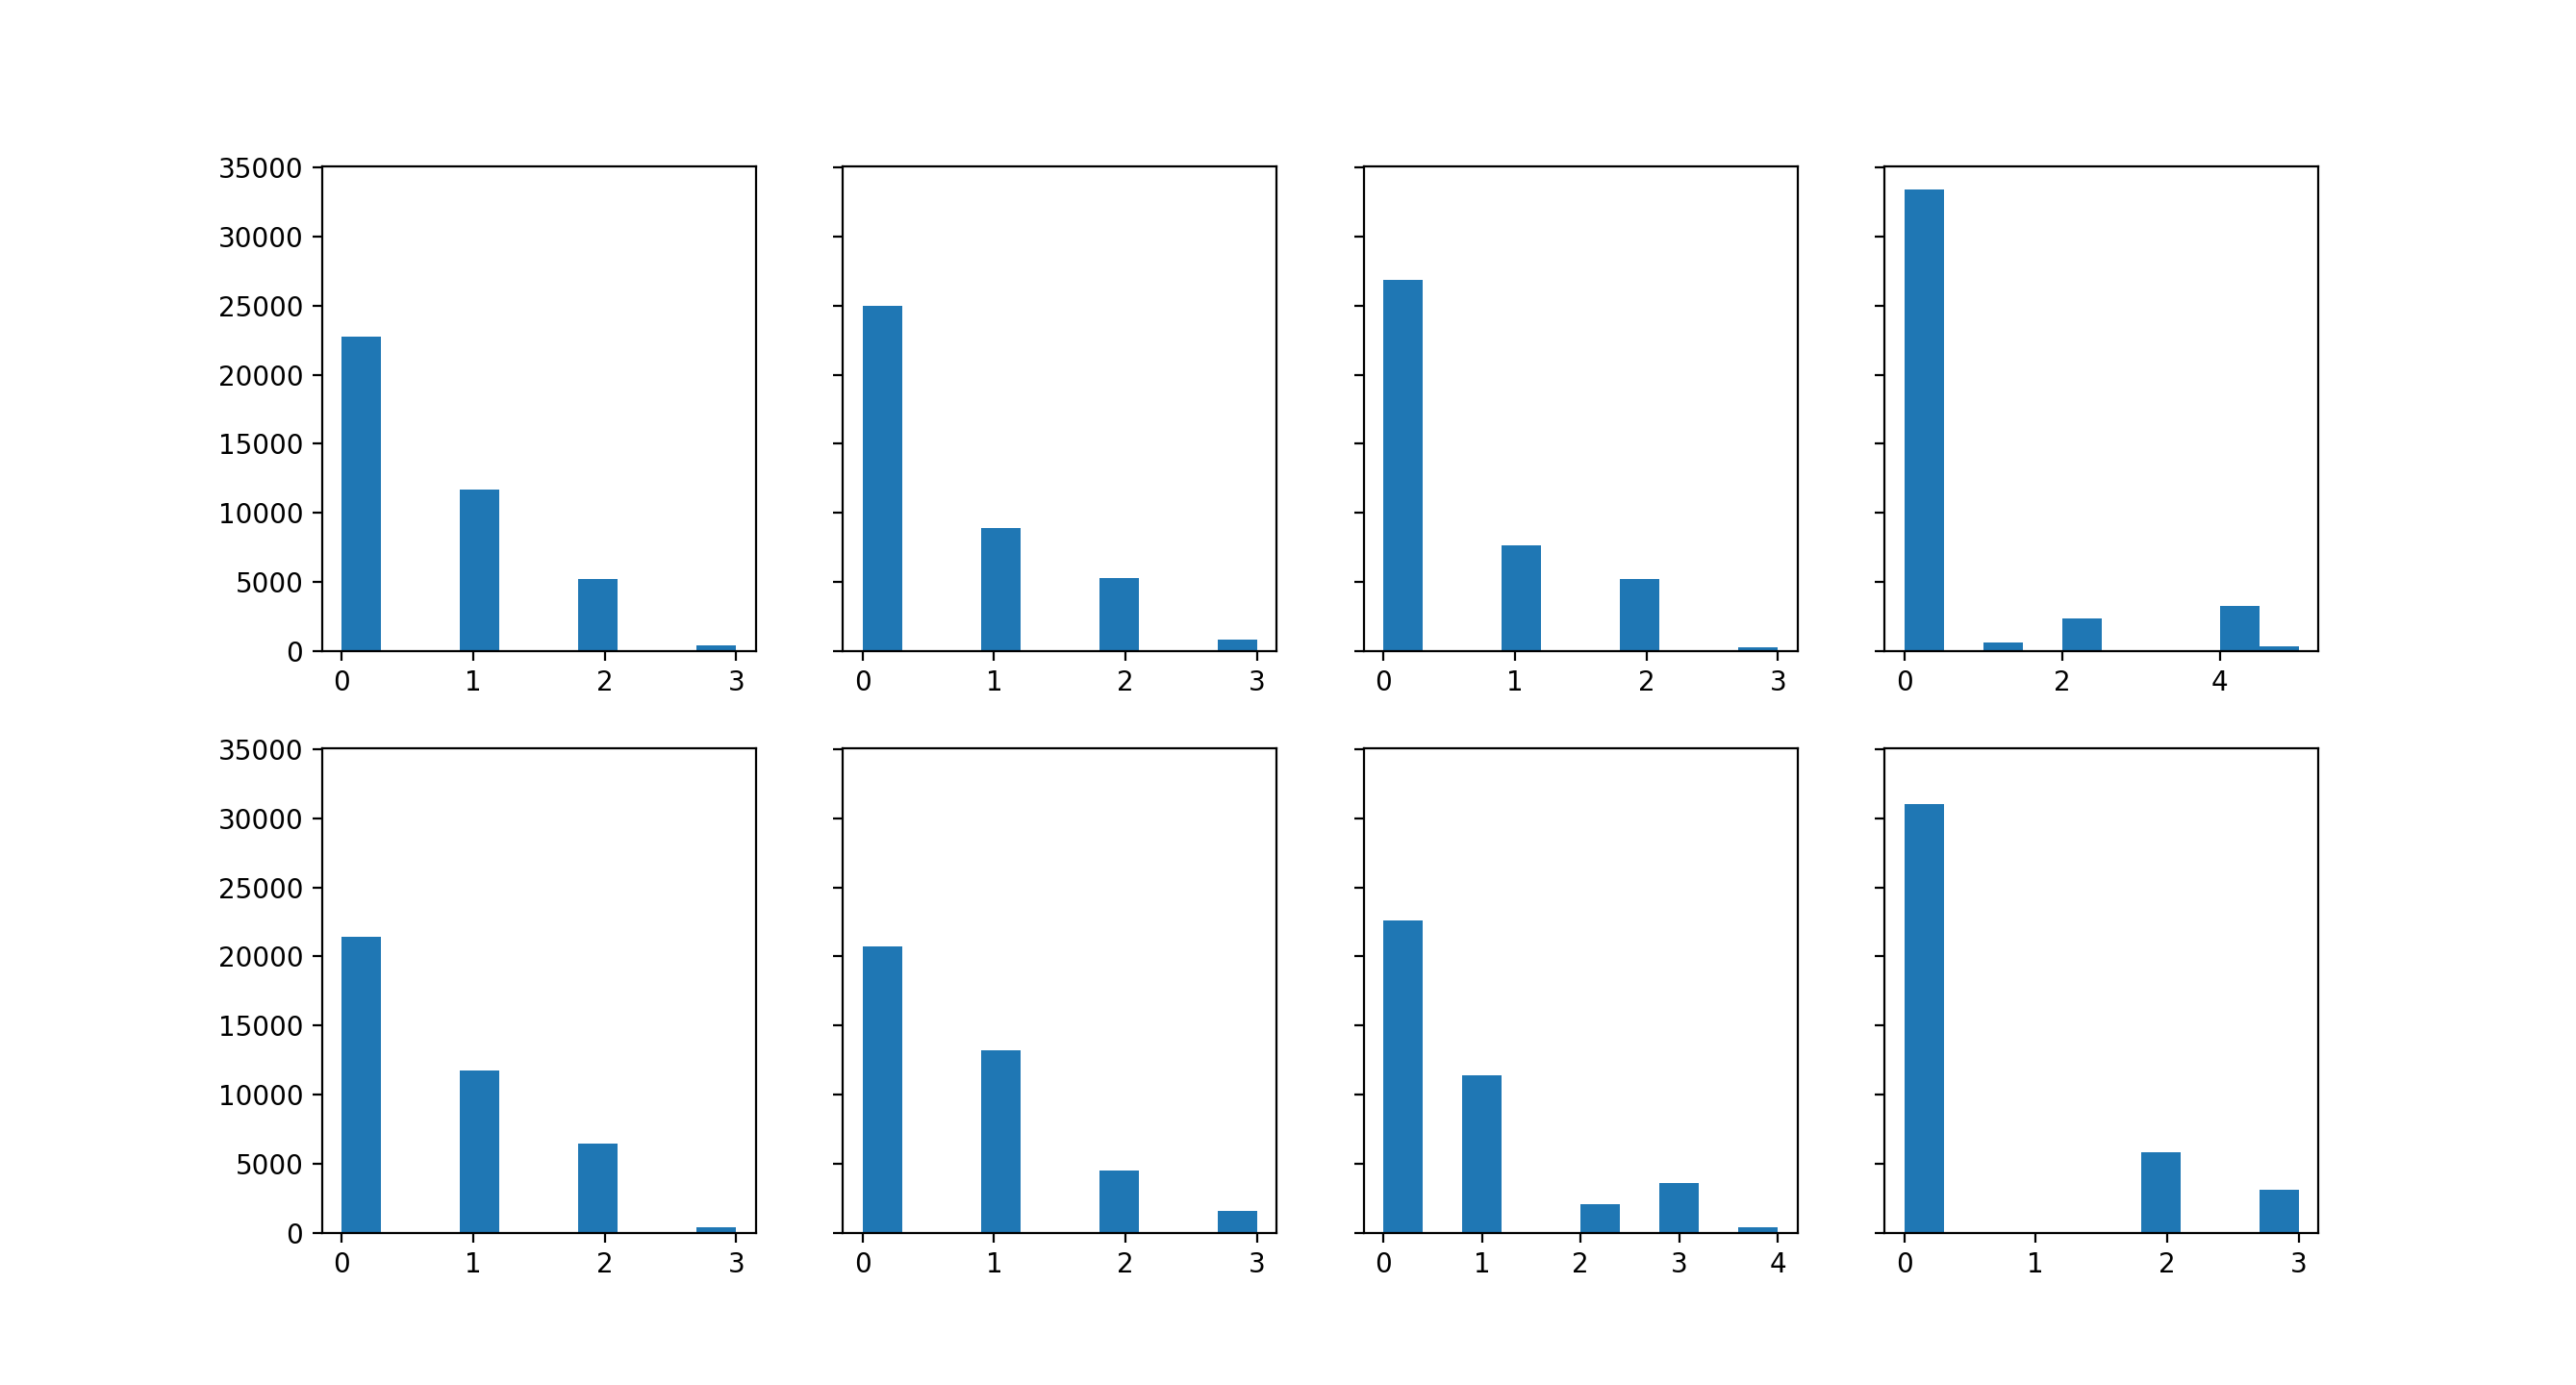
\includegraphics[width=\linewidth]{matplotlibPlots/effectRegionCounts.png}
  		\caption{(PLACEHOLDER)}
		\label{fig:counts}
	\end{center}
\end{figure}

\begin{figure}[h!tb]
	\begin{center}
  		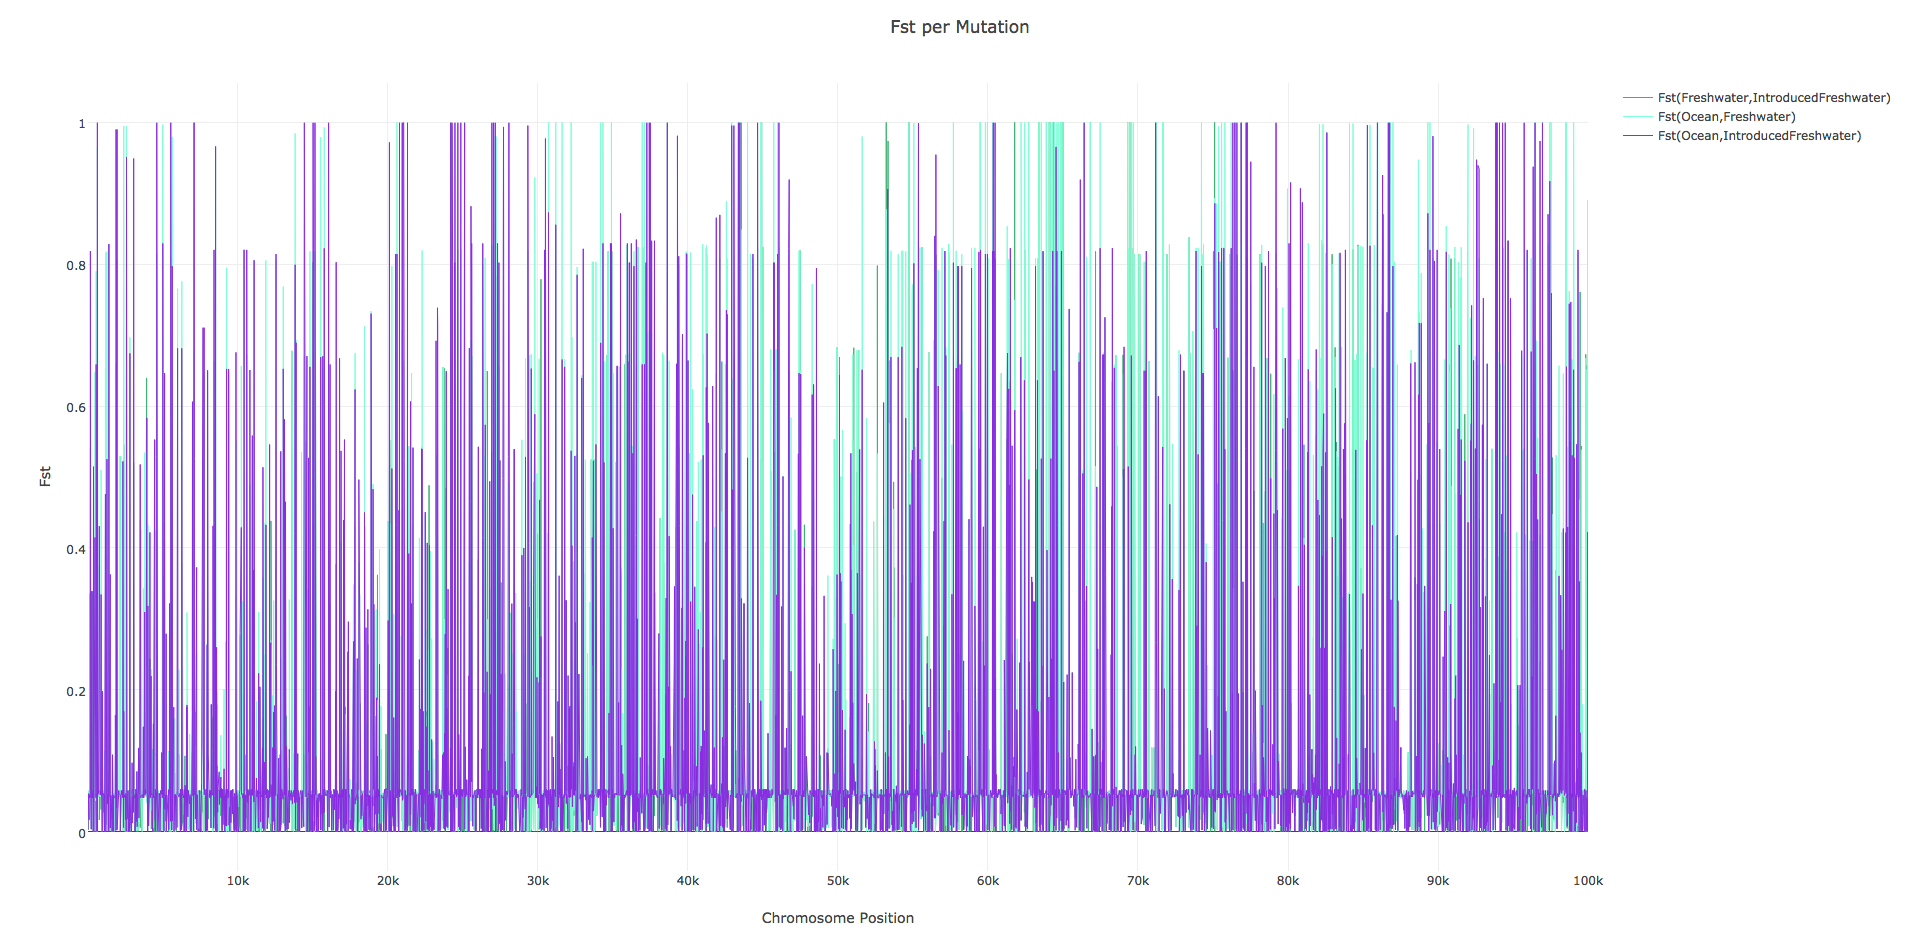
\includegraphics[width=0.7\linewidth]{plotlyPlots/FstAcross5e-5.png}
  		\caption{ (PLACEHOLDER)
		}
  		\label{fig:Fst1}
	\end{center}
\end{figure}

\begin{figure}[h!tb]
	\begin{center}
  		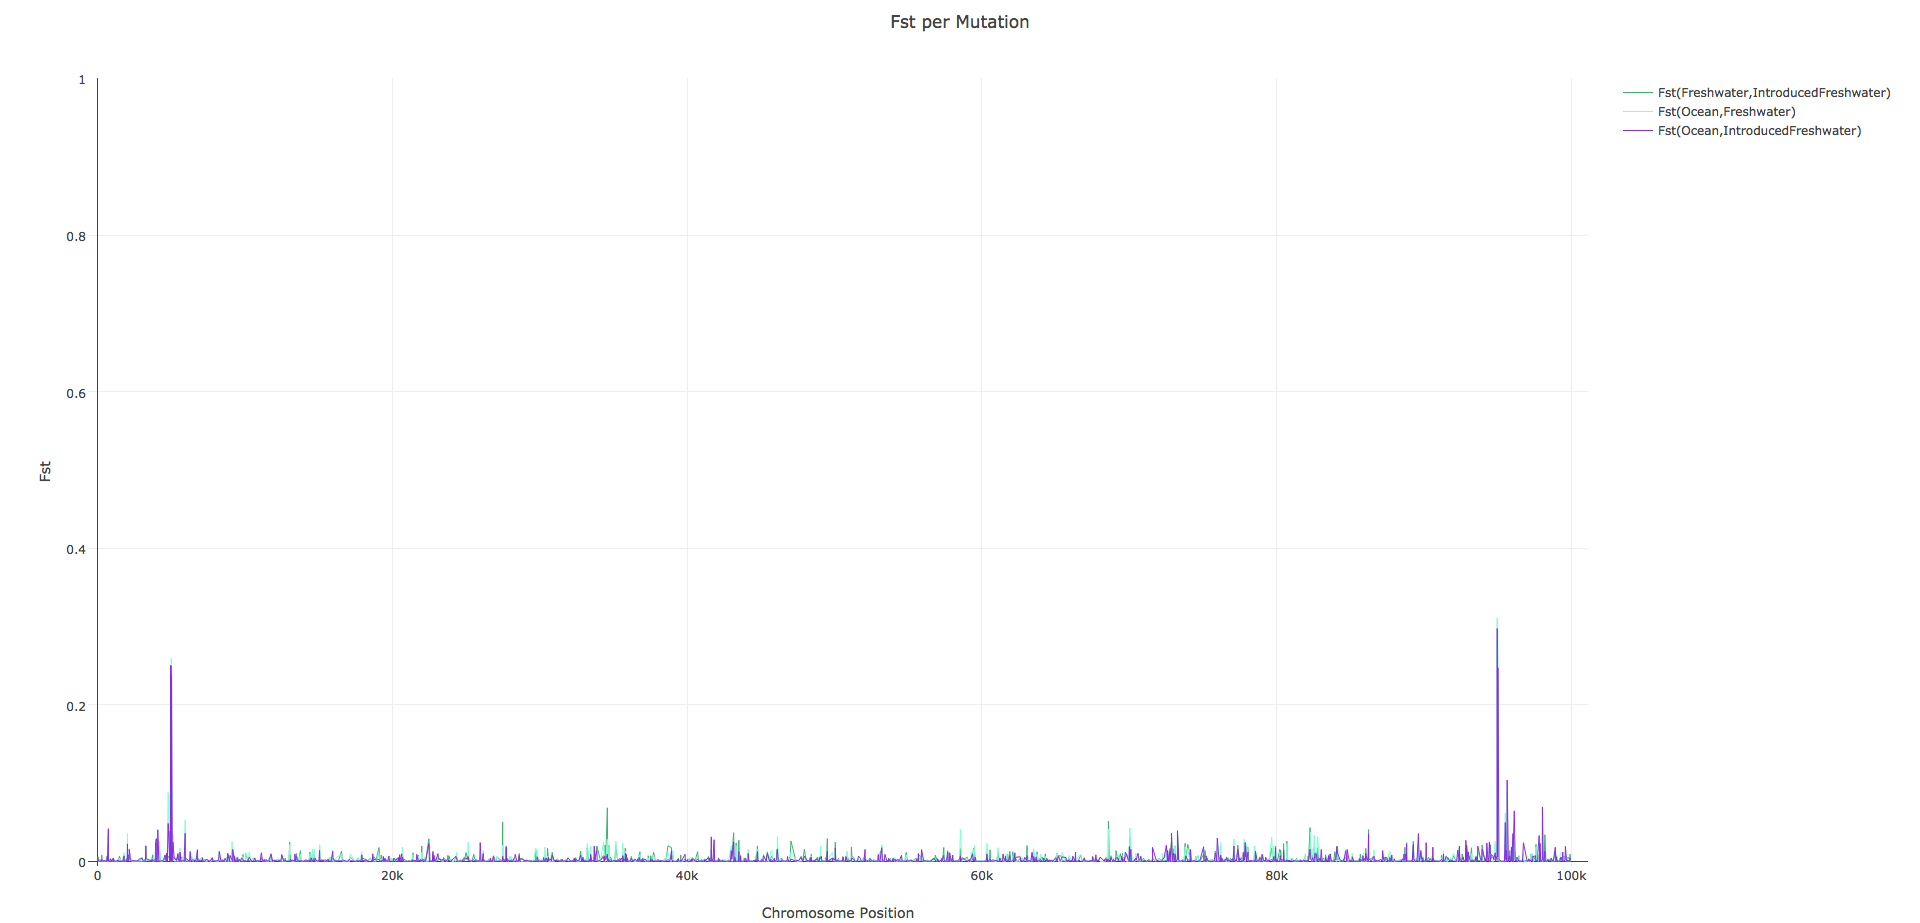
\includegraphics[width=0.7\linewidth]{plotlyPlots/FstAcross5e-2.png}
  		\caption{(PLACEHOLDER)
		}
  		\label{fig:Fst4}
	\end{center}
\end{figure}

\begin{figure}[h!tb]
	\begin{center}
  		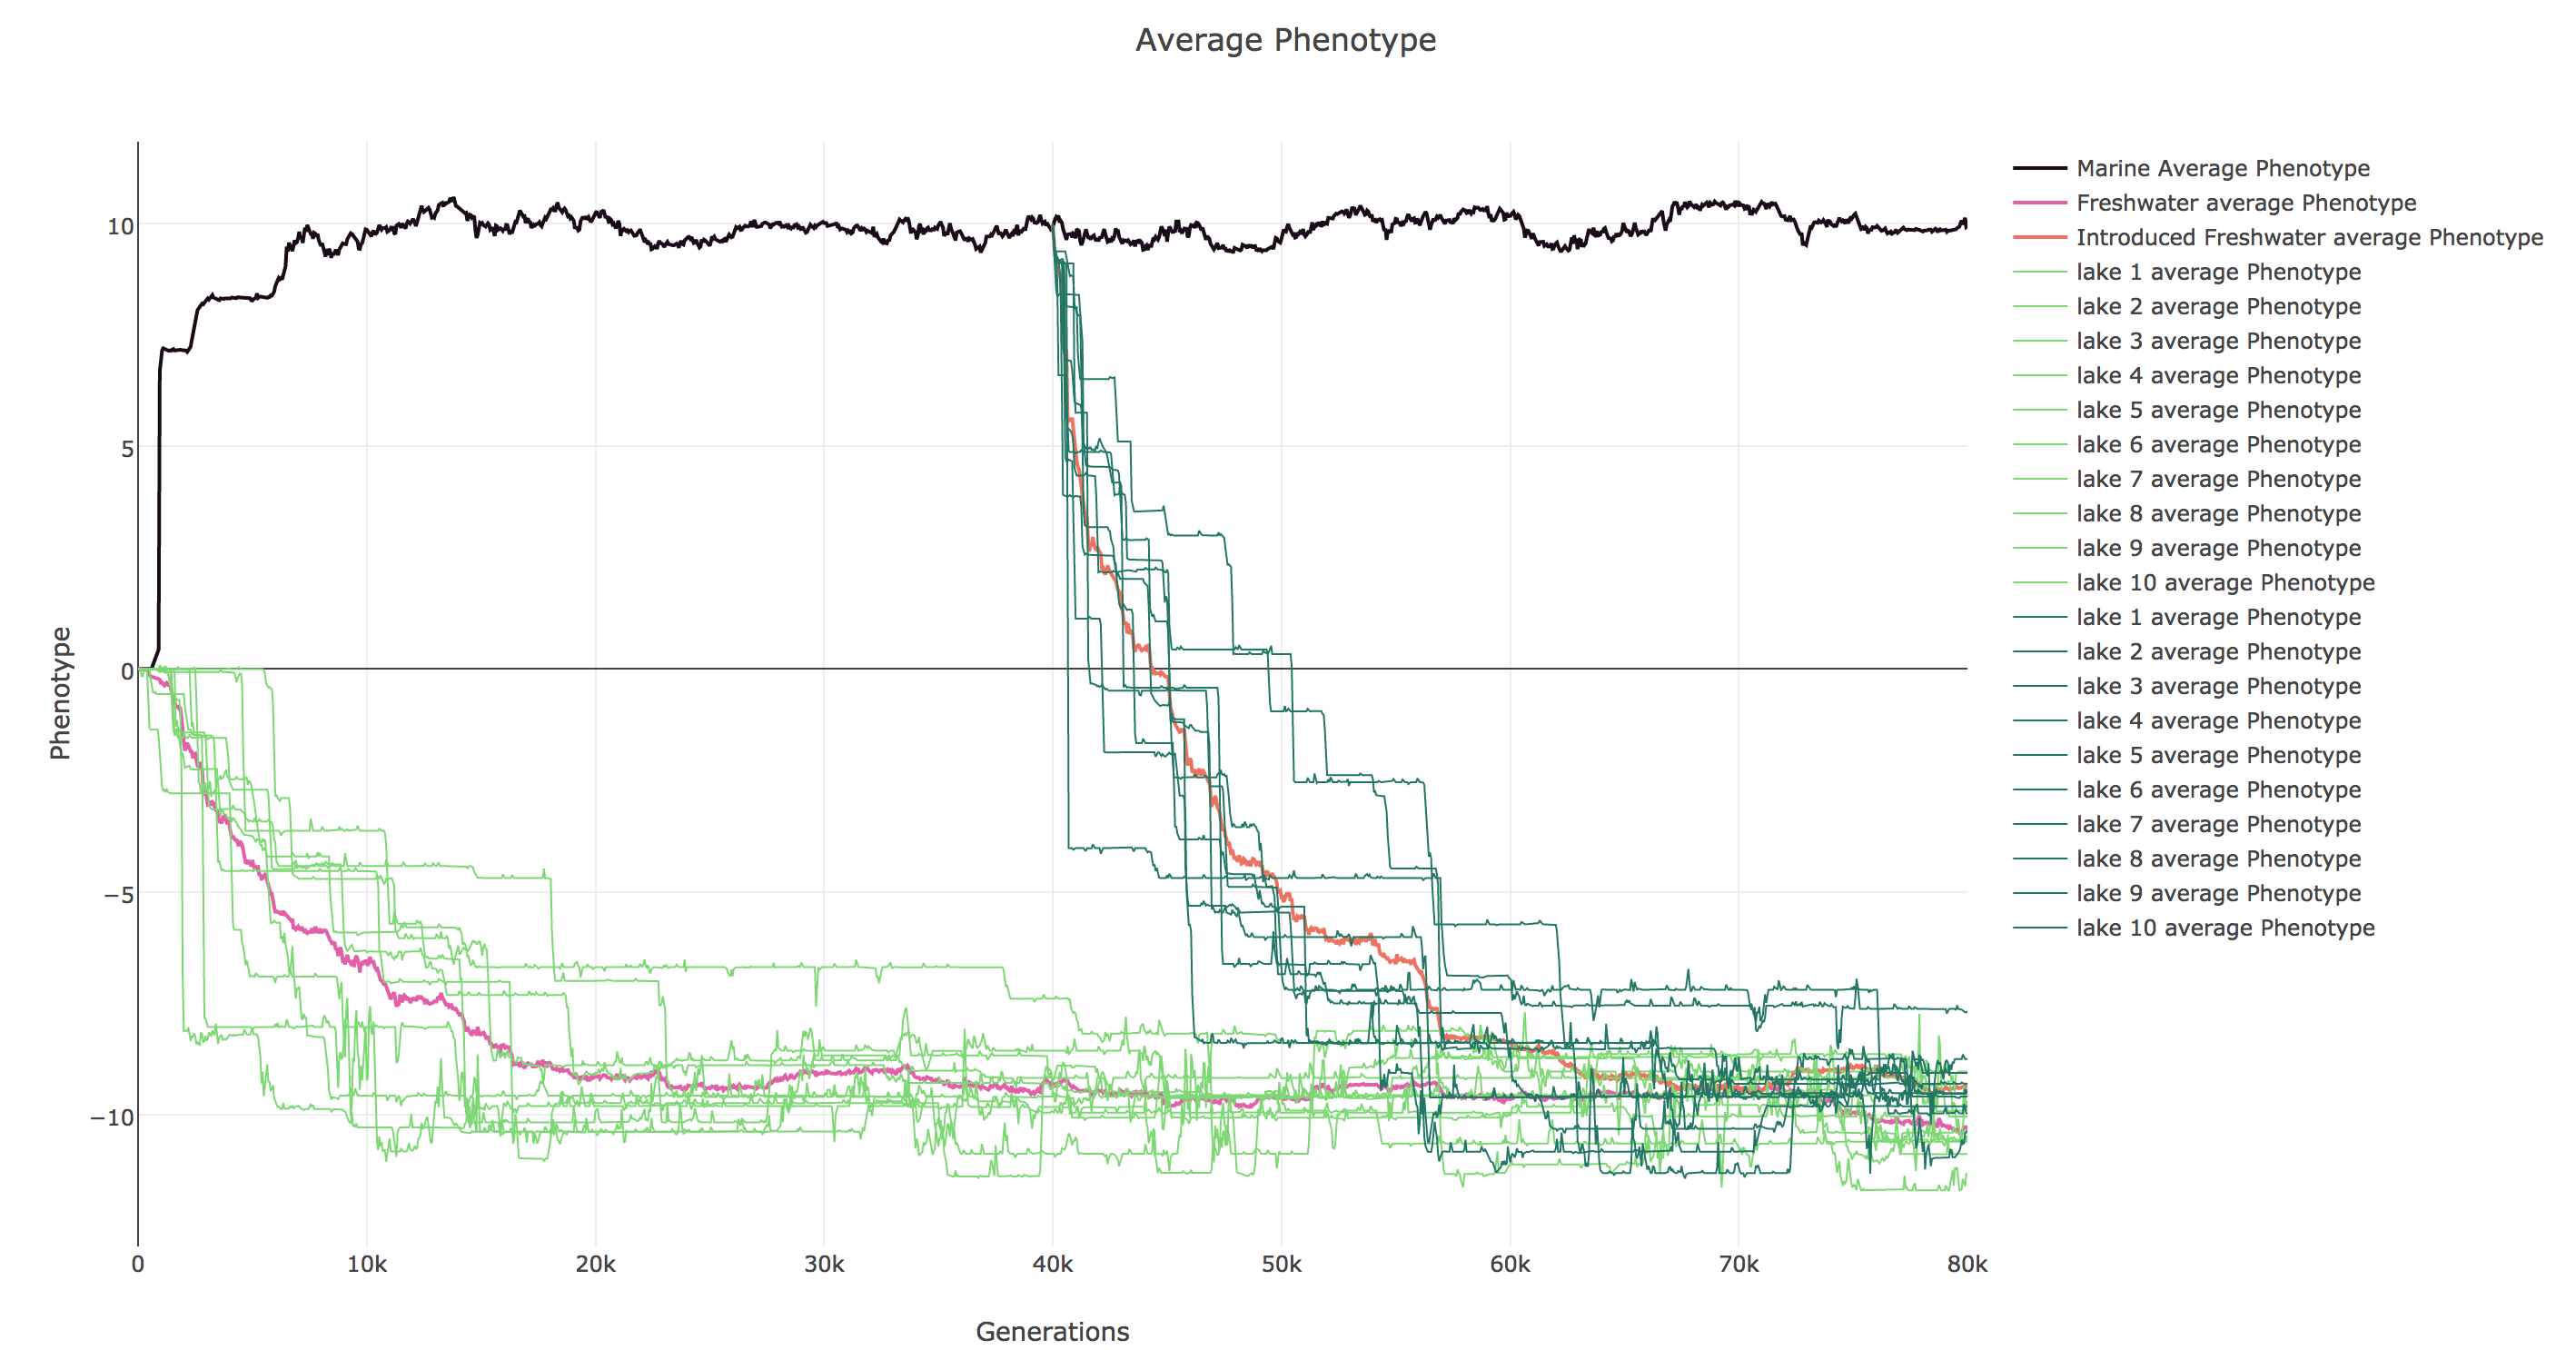
\includegraphics[width=0.7\linewidth]{plotlyPlots/PhenotypeThroughout5e-5.png}
  		\caption{ (PLACEHOLDER)
		}
  		\label{fig:phenotype_ts1}
	\end{center}
\end{figure}

\begin{figure}[h!tb]
	\begin{center}
  		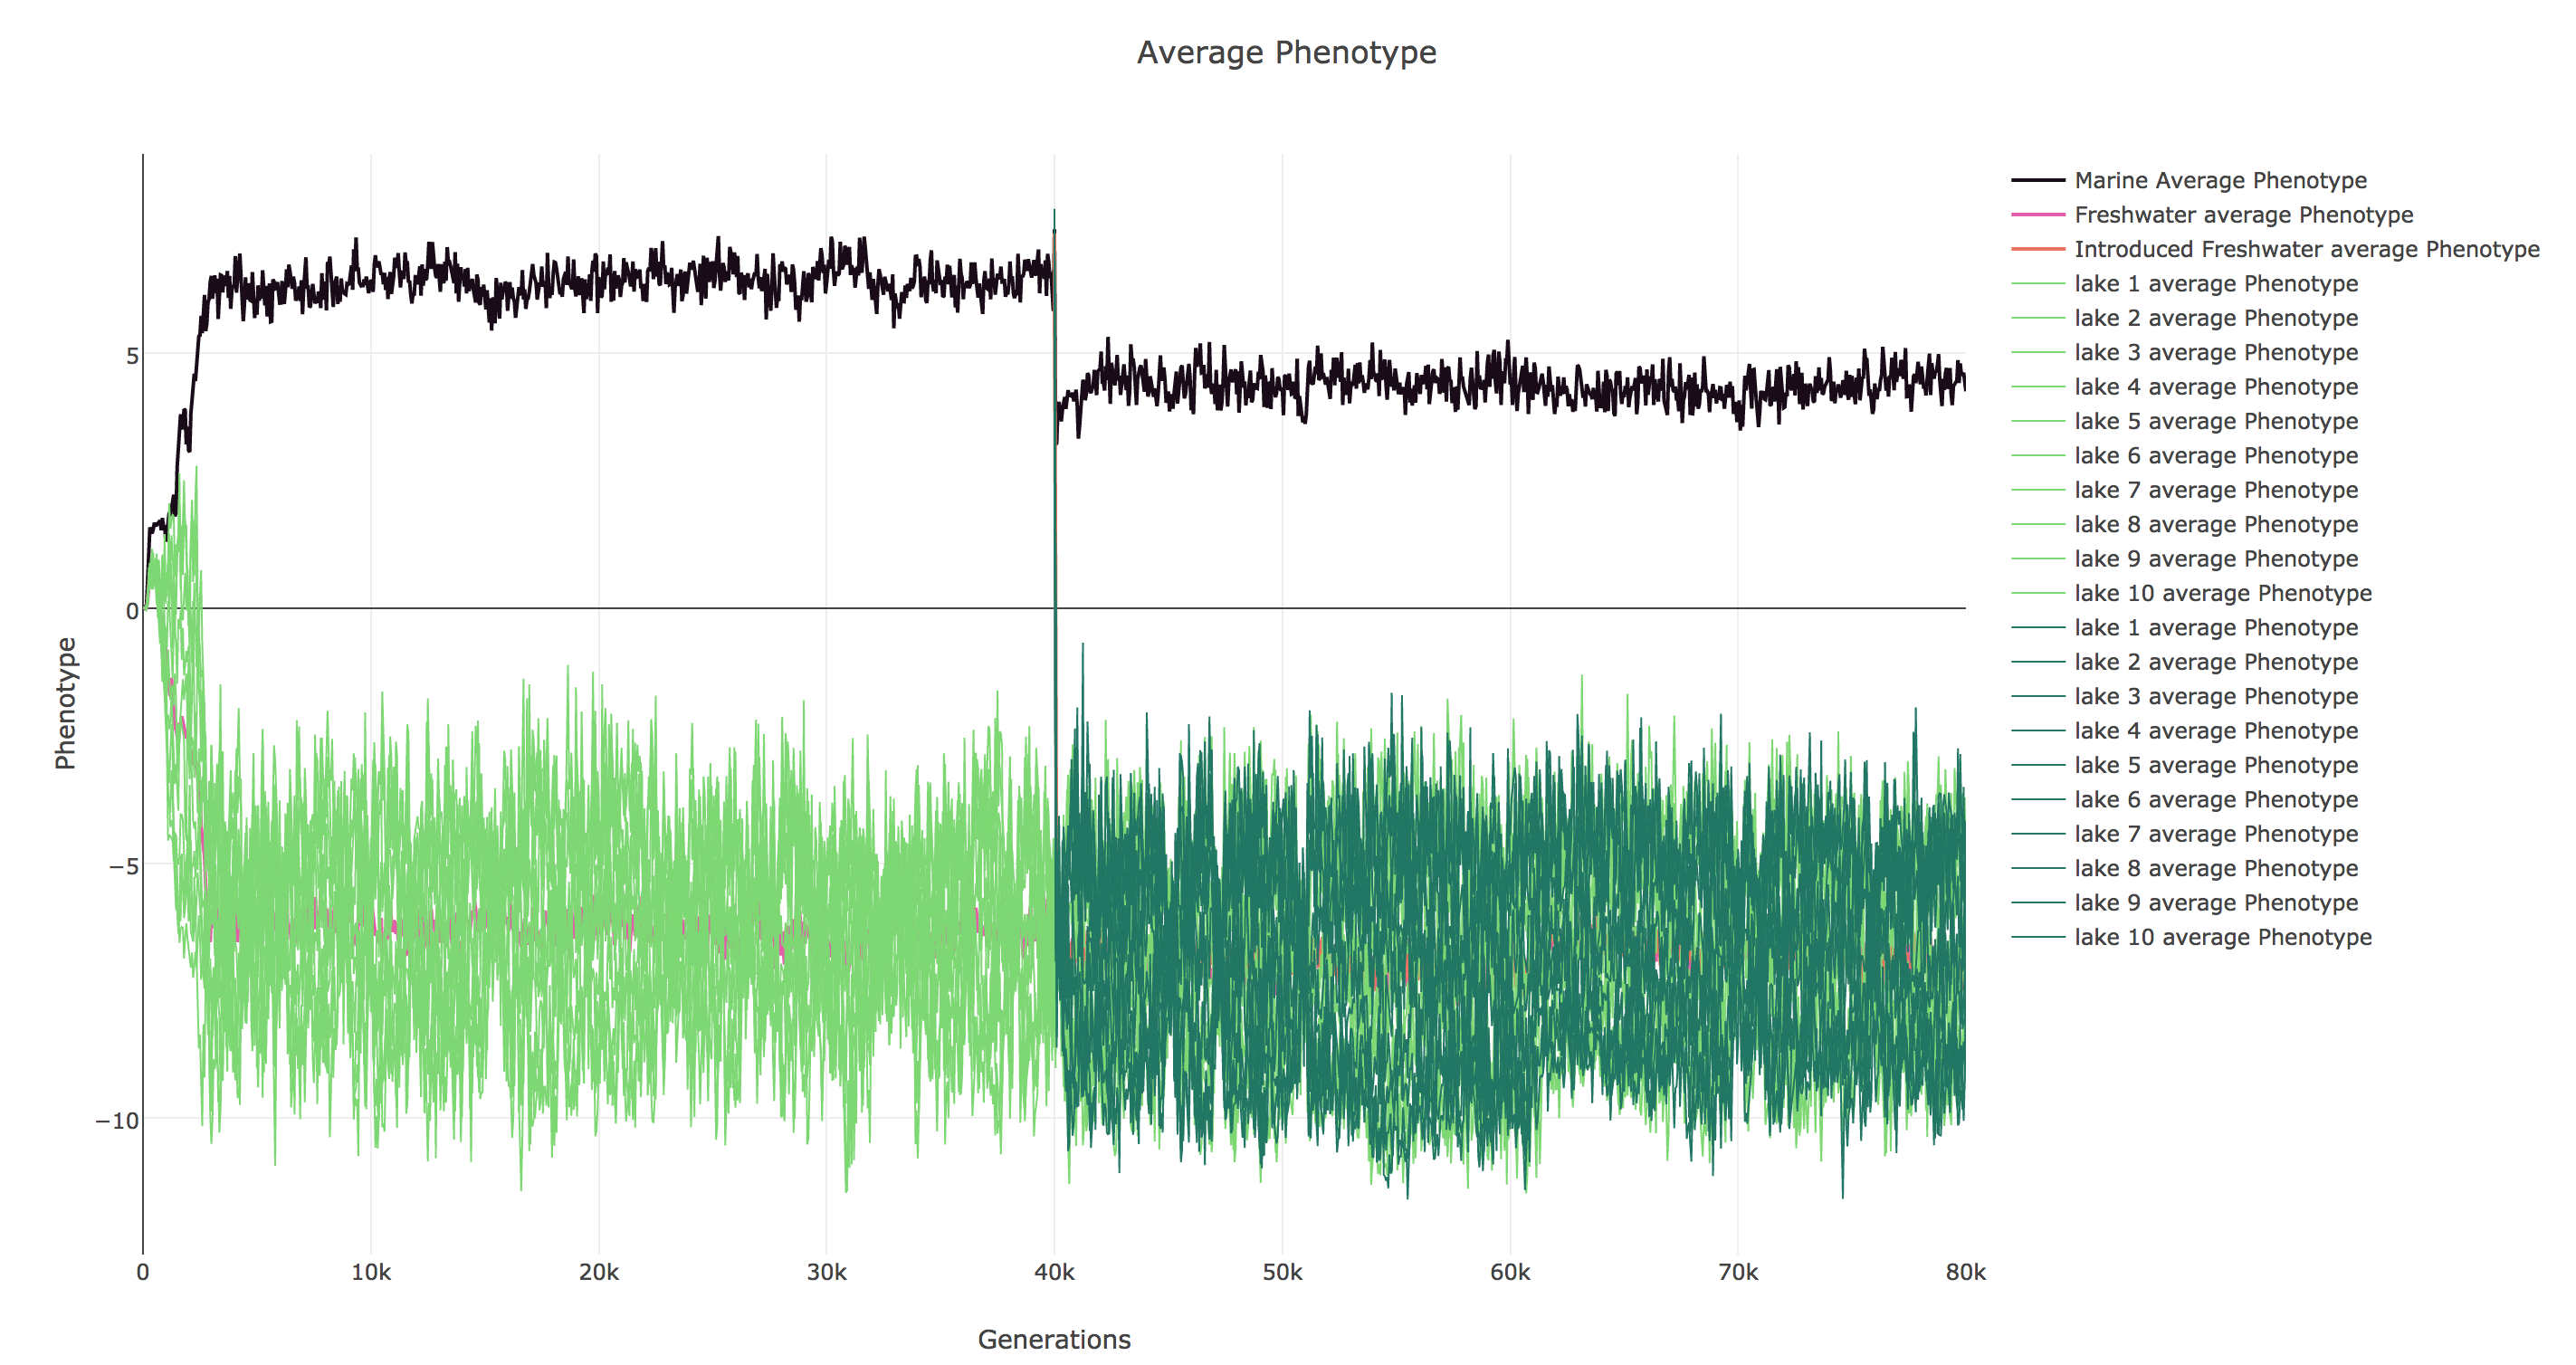
\includegraphics[width=0.7\linewidth]{plotlyPlots/PhenotypeThroughout5e-2.png}
  		\caption{(PLACEHOLDER)
		}
  		\label{fig:phenotype_ts4}
	\end{center}
\end{figure}



\end{document}
